\documentclass[12pt, a4paper]{article}

\usepackage[utf8]{inputenc}
\usepackage[german]{babel}
\usepackage{lmodern}
\usepackage[T1]{fontenc}
\usepackage{amsmath, amssymb, amsthm, mathtools}
\usepackage{geometry}
\usepackage{graphicx}
\usepackage{float}
\usepackage{caption}
\usepackage{subcaption}
\usepackage{booktabs}
\usepackage{array}
\usepackage{xcolor}
\usepackage{hyperref}
\usepackage{enumitem}
\usepackage{setspace}
\usepackage{fancyhdr}
\usepackage{titlesec}
% \usepackage{microtype}
\usepackage{bm}
\usepackage{physics}
\usepackage{tikz}
\usetikzlibrary{arrows.meta, decorations.pathmorphing, patterns, shapes.geometric, positioning, calc}

\emergencystretch=1.5em

\geometry{margin=2.5cm}

\hypersetup{
  colorlinks=true,
  linkcolor=blue!55!black,
  citecolor=green!55!black,
  urlcolor=blue!55!black,
  pdftitle={Harmonische Ausbreitung akustischer Signale in symmetrischen Hörräumen}
}

% ============================================================
% THEOREM-UMGEBUNGEN
% ============================================================
\theoremstyle{definition}
\newtheorem{definition}{Definition}[section]
\newtheorem{satz}{Satz}[section]
\newtheorem{lemma}{Lemma}[section]
\newtheorem{korollar}{Korollar}[section]
\newtheorem{beispiel}{Beispiel}[section]
\newtheorem{bemerkung}{Bemerkung}[section]
\newtheorem{theorem}{Theorem}[section]

\theoremstyle{remark}
\newtheorem*{beweis*}{Beweis}

% ============================================================
% MAKROS
% ============================================================
\newcommand{\R}{\mathbb{R}}
\newcommand{\C}{\mathbb{C}}
\newcommand{\N}{\mathbb{N}}
\newcommand{\Lx}{L_x}
\newcommand{\Ly}{L_y}
\newcommand{\Lz}{L_z}
\newcommand{\kv}{\mathbf{k}}
\newcommand{\xv}{\mathbf{x}}
\renewcommand{\norm}[1]{\left\| #1 \right\|}
\renewcommand{\abs}[1]{\left| #1 \right|}
\newcommand{\pfrac}[2]{\frac{\partial #1}{\partial #2}}
\DeclareMathOperator{\sgn}{sgn}

\title{\textbf{Harmonische Ausbreitung akustischer Signale in symmetrischen Hörräumen}\\
Theoretische Grundlagen, formale Nachweise und raumakustische Konsequenzen}
\date{13. April 2026}
\author{Stephan Epp}

\begin{document}

\maketitle
\tableofcontents
\newpage

% ============================================================
\section{Einleitung und Motivation}
% ============================================================
Diese Arbeit untersucht die harmonische Ausbreitung akustischer Signale in geometrisch
symmetrischen Hörräumen, insbesondere in rechteckigen Quader- und Hörsälen. Im Zentrum
steht die Frage, wie weit sich aus der Symmetrie eines Raumes belastbare Aussagen über
Eigenmoden, Eigenfrequenzen, Schalldruckverteilungen und raumakustische Gütekriterien
ableiten lassen. Dabei wird die Raumakustik nicht nur als Berechnung einzelner Frequenzen
verstanden, sondern als zusammenhängendes Problem aus Wellenausbreitung, Spektraltheorie,
Geometrie, Messung und Wahrnehmung.

Ausgehend von der Wellengleichung werden zunächst die Randbedingungen des symmetrischen
Raumes hergeleitet, die Eigenmoden klassifiziert und ihre Frequenzrelationen untersucht.
Die exakten harmonischen Reihen der axialen Moden werden dabei von den nur unter
zusätzlichen Voraussetzungen rationalen Frequenzverhältnissen allgemeiner Moden
unterschieden. Diese Unterscheidung ist wichtig, weil geometrische Symmetrie allein
nicht garantiert, dass das gesamte dreidimensionale Spektrum aus ganzzahligen Vielfachen
einer einzigen Grundfrequenz besteht. Die Greensche Funktion des symmetrischen Raumes
wird anschließend konstruiert und ihre Spiegeleigenschaften werden formal nachgewiesen.
Darauf aufbauend werden Nachhallzeit, C50, D50 und die räumliche Gleichmäßigkeit des
Schallfeldes als anwendungsnahe Kriterien eingeführt.

Die Arbeit verbindet diese mathematisch-physikalische Analyse mit numerischen
Illustrationen und einer biologisch-neurowissenschaftlichen Erweiterung. Das in Kapitel
9 ergänzte Kapitel untersucht, wie ITD, ILD, cochleäre Frequenzselektion, neuronale
Synchronisation und bewegliche Ohrmuscheln die auditive Raumorientierung beeinflussen.
Damit wird die Perspektive vom Raum als physikalischem System auf die Wechselwirkung
zwischen Schallfeld und Empfänger erweitert: Ein Hörsaal kann akustisch symmetrisch
sein, während ein realer Zuhörer die resultierende Symmetrie aufgrund individueller
Hörschwellen, HRTFs und kognitiver Verarbeitung unterschiedlich erlebt.

Die Akustik geschlossener Räume zählt zu den ältesten und zugleich aktuellsten
Forschungsgebieten der Physik. Von den griechischen Amphitheatern über
die gotischen Kathedralen bis hin zu modernen Konzertsälen und universitären
Hörsälen stellte und stellt die Frage nach der optimalen Schallverteilung
eine zentrale ingenieurtechnische und wissenschaftliche Herausforderung dar.

Symmetrische Hörräume --- also Räume, die eine oder mehrere geometrische
Symmetrieachsen oder -ebenen aufweisen --- nehmen in dieser Betrachtung
eine besondere Stellung ein. Die geometrische Symmetrie pflanzt sich
unmittelbar in die Physik der Schallausbreitung fort: Randbedingungen,
Eigenmoden und Greenssche Funktion erben die Symmetrieeigenschaften des
umgebenden Gebiets. Die zentrale Aussage dieser Arbeit lautet:

\begin{center}
\textit{In einem geometrisch symmetrischen Hörsaal breitet sich Schall
harmonisch aus --- das heißt, die Eigenfrequenzen bilden rationale
Vielfache einer Grundfrequenz, und die Schalldruckverteilung besitzt
die gleiche Symmetriegruppe wie der Raum selbst.}
\end{center}

Diese Aussage wird in den folgenden Kapiteln mathematisch präzisiert, formal
bewiesen, numerisch geprüft und im Hinblick auf Wahrnehmung und Anwendung eingeordnet.
Die leitenden Forschungsfragen lauten:

\begin{enumerate}
\item Welche Randbedingungen und Symmetrieoperationen bestimmen die Eigenmoden eines
  schallharten Quaderaums?
\item Unter welchen geometrischen Voraussetzungen entstehen exakte harmonische Reihen,
  und wann sind lediglich quasi-harmonische oder statistische Strukturen zu erwarten?
\item Wie übertragen sich Symmetrien von den Eigenmoden und der Greenschen Funktion
  auf messbare Größen wie Schalldruck, Nachhall und Sprachverständlichkeit?
\item Wie verändern Absorption, Temperaturgradienten, Geometrieabweichungen und aktive
  Lautsprecher die idealen Symmetrieaussagen?
\item Welche zusätzlichen Bedingungen entstehen, wenn nicht nur das Schallfeld,
  sondern auch das menschliche oder tierische Hörsystem als Empfänger modelliert wird?
\end{enumerate}

Zur Beantwortung dieser Fragen folgt die Arbeit einer gestuften Methodik. Zuerst werden
analytische Modelle und Beweise für den idealisierten Quader entwickelt. Danach werden
die Ergebnisse mit numerischen Darstellungen der Moden, Greenschen Funktion und
raumakustischen Kennwerte veranschaulicht. Kapitel 8 erweitert diese Beschreibung um
psychoakustische und biologische Größen, bevor im abschließenden Ausblick beide Ebenen
zusammengeführt werden. Der abschließende Ausblick führt die physikalische Analyse und
die Wahrnehmungs- sowie Biologieperspektive zusammen und benennt konkrete Wege zur
experimentellen Validierung und technischen Umsetzung. Die Arbeit beansprucht dabei
keine vollständige Simulation realer Hörsäle; ihre Stärke liegt in der transparenten
Verbindung von Modellannahmen, Folgerungen und klar benannten Grenzen.

Dabei werden folgende Aspekte systematisch behandelt:

\begin{enumerate}
\item Die Wellengleichung als Ausgangspunkt und ihre Randbedingungen
  im Quaderraum (Abschnitt~\ref{sec:wellengleichung});
\item Die vollständige Herleitung und Klassifikation der Eigenmoden
  des symmetrischen Hörsaals (Abschnitt~\ref{sec:eigenmoden});
\item Der formale Nachweis der harmonischen Struktur des Eigenfrequenz\-spektrums
  (Abschnitt~\ref{sec:harmonik});
\item Die Konstruktion der Greenschen Funktion und ihre Symmetrieeigenschaften
  (Abschnitt~\ref{sec:greens});
\item Raumakustische Gütekriterien und ihre Abhängigkeit von der Symmetrie
  (Abschnitt~\ref{sec:raumakustik});
\item Numerische Illustrationen aller theoretischen Ergebnisse
  (Abschnitt~\ref{sec:simulation});
\item Eine biologische und neurowissenschaftliche Einordnung von Hörwahrnehmung,
  Raumorientierung und den besonderen Eigenschaften des felinen Gehörs
  (Abschnitt~\ref{sec:biologie});
\item Der abschließende Rückblick mit Zusammenfassung, Ausblick und der
  Einordnung offener theoretischer, numerischer, biologischer und technischer
  Forschungsfragen (Abschnitt~\ref{sec:ausblick}).
\end{enumerate}

\subsection*{Konventionen und Notation}

Vektoren werden fett gedruckt: $\mathbf{x} = (x,y,z)^\top \in \R^3$.
Der Schallwellenoperator lautet $\Box = \Delta - \frac{1}{c^2}\partial_{tt}$,
wobei $c \approx 343\,\mathrm{m/s}$ die Schallgeschwindigkeit in Luft bei
$20\,^\circ\mathrm{C}$ bezeichnet. Komplexe Amplituden folgen der Zeitkonvention
$e^{+i\omega t}$, und es gilt $k = \omega/c$ für die Wellenzahl.

\textit{\textbf{Schlüsselwörter}}: Raumakustik, Wellengleichung, Eigenmoden,
harmonische Reihen, symmetrische Räume, Greensche Funktion, Nachhallzeit,
Fourier-Analyse, Geometrische Akustik

% ============================================================
\section{Die Wellengleichung und ihre Randbedingungen}
\label{sec:wellengleichung}
% ============================================================

\subsection{Akustische Grundgleichungen}

Die lineare Akustik eines idealen, kompressiblen Fluids wird durch drei
Grundgleichungen beschrieben. Sei $\rho_0$ die Ruhedichte und $\kappa$
der isentrope Kompressionsmodul der Luft.

\begin{definition}[Akustische Zustandsgrößen]
Der Schalldruck $p(\mathbf{x},t) \in \R$, die Schallschnelle
$\mathbf{v}(\mathbf{x},t) \in \R^3$ und die Dichteschwankung
$\rho'(\mathbf{x},t) \in \R$ sind die linearisierten Schwankungsgrößen
um den Ruhezustand $(\rho_0, \mathbf{0}, p_0)$.
\end{definition}

Die linearisierten Euler-Gleichungen lauten:
\begin{align}
  \rho_0 \pfrac{\mathbf{v}}{t} &= -\nabla p,
  \label{eq:euler}\\[6pt]
  \pfrac{\rho'}{t} + \rho_0\, \nabla \cdot \mathbf{v} &= Q(\mathbf{x},t),
  \label{eq:kontinuitaet}\\[6pt]
  p &= c^2 \rho',
  \label{eq:zustand}
\end{align}
wobei $Q$ eine externe Quelldichte bezeichnet und
$c^2 = \kappa / \rho_0$ gilt.

Durch Elimination von $\mathbf{v}$ und $\rho'$ ergibt sich unmittelbar:

\begin{satz}[Inhomogene Wellengleichung]
\label{satz:welle}
Unter den obigen Annahmen genügt der Schalldruck $p$ der inhomogenen
Wellengleichung
\begin{equation}
  \Box\, p(\mathbf{x},t) \;:=\;
  \Delta p(\mathbf{x},t) - \frac{1}{c^2}\,\pfrac{^2 p}{t^2}(\mathbf{x},t)
  \;=\; -\rho_0 \pfrac{Q}{t}(\mathbf{x},t).
  \label{eq:wellengl}
\end{equation}
\end{satz}

\begin{proof}
Wir differenzieren Gleichung~\eqref{eq:euler} nach der Zeit:
$\rho_0 \partial_{tt} \mathbf{v} = -\nabla\,\partial_t p.$
Die Divergenz von~\eqref{eq:euler} ergibt
$\rho_0 \partial_t (\nabla \cdot \mathbf{v}) = -\Delta p.$
Aus der Kontinuitätsgleichung~\eqref{eq:kontinuitaet} folgt
$\partial_t \rho' = \rho_0 Q - \rho_0 \nabla\cdot\mathbf{v}$,
also $\partial_{tt}\rho' = -\rho_0(\partial_t Q - \partial_t\nabla\cdot\mathbf{v}).$
Mit~\eqref{eq:zustand} und der Elimination von $\nabla\cdot\mathbf{v}$ folgt
\[
  \frac{1}{c^2}\partial_{tt} p = \Delta p - \rho_0\, \partial_t Q,
\]
was~\eqref{eq:wellengl} entspricht. 
\end{proof}

\subsection{Harmonischer Ansatz und Helmholtz-Gleichung}

Für periodische Anregung mit Kreisfrequenz $\omega$ setzen wir den Produktansatz
\[
  p(\mathbf{x},t) = \Re\!\left[\hat{p}(\mathbf{x})\,e^{+i\omega t}\right]
\]
ein und erhalten:

\begin{satz}[Helmholtz-Gleichung]
Die komplexe Druckamplitude $\hat{p}(\mathbf{x})$ genügt der
Helmholtz-Gleichung
\begin{equation}
  (\Delta + k^2)\,\hat{p}(\mathbf{x}) = -\hat{Q}(\mathbf{x}),
  \qquad k = \frac{\omega}{c},
  \label{eq:helmholtz}
\end{equation}
wobei $\hat{Q}$ die komplexe Quellstärke bezeichnet.
\end{satz}

\subsection{Randbedingungen am symmetrischen Quaderraum}

Sei $\Omega = (0,\Lx) \times (0,\Ly) \times (0,\Lz) \subset \R^3$
der Hörsaal mit schallharten Wänden. Die Neumann-Randbedingung
\begin{equation}
  \left.\pfrac{\hat{p}}{\mathbf{n}}\right|_{\partial\Omega} = 0
  \label{eq:rbc}
\end{equation}
modelliert vollständige Reflexion ($\mathbf{n}$: äußere Einheitsnormale).

\begin{definition}[Symmetrischer Hörsaal]
\label{def:sym_hoersaal}
Ein Quaderraum $\Omega = (0,\Lx)\times(0,\Ly)\times(0,\Lz)$ heißt
\emph{geometrisch symmetrisch}, wenn mindestens eine der folgenden
Spiegelsymmetrien gilt:
\begin{enumerate}[label=(\roman*)]
\item $x \mapsto \Lx - x$ (Spiegelung an $x = \Lx/2$),
\item $y \mapsto \Ly - y$ (Spiegelung an $y = \Ly/2$),
\item $z \mapsto \Lz - z$ (Spiegelung an $z = \Lz/2$).
\end{enumerate}
\end{definition}

Der typische universitäre Hörsaal erfüllt alle drei Symmetrien. Im Folgenden
betrachten wir den vollständig symmetrischen Fall.

% ============================================================
\section{Eigenmoden des symmetrischen Hörsaals}
\label{sec:eigenmoden}
% ============================================================

\subsection{Herleitung durch Separation der Variablen}

Mit dem Produktansatz $\hat{p}(\mathbf{x}) = X(x)\,Y(y)\,Z(z)$ zerfällt
die Helmholtz-Gleichung~\eqref{eq:helmholtz} im quellfreien Fall in drei
gewöhnliche Differentialgleichungen.

\begin{satz}[Separation]
\label{satz:separation}
Die Lösungen von $(\Delta + k^2)\hat{p} = 0$ in $\Omega$ mit
Randbedingung~\eqref{eq:rbc} sind von der Form
\begin{equation}
  \hat{p}_{mnl}(\mathbf{x}) = A_{mnl}\,
  \cos\!\left(\frac{m\pi x}{\Lx}\right)
  \cos\!\left(\frac{n\pi y}{\Ly}\right)
  \cos\!\left(\frac{l\pi z}{\Lz}\right),
  \label{eq:moden}
\end{equation}
mit $m,n,l \in \N_0 = \{0,1,2,\ldots\}$, $(m,n,l) \neq (0,0,0)$.
\end{satz}

\begin{proof}
Mit dem Ansatz $\hat{p} = X(x)Y(y)Z(z)$ ergibt sich nach Division durch $XYZ$:
\[
  \underbrace{\frac{X''}{X}}_{=:-k_x^2}
  + \underbrace{\frac{Y''}{Y}}_{=:-k_y^2}
  + \underbrace{\frac{Z''}{Z}}_{=:-k_z^2}
  = -k^2.
\]
Für jede Koordinate gilt z.\,B. $X'' + k_x^2 X = 0$ mit allgemeiner Lösung
$X(x) = C_1\cos(k_x x) + C_2\sin(k_x x)$.
Die Randbedingung $X'(0) = 0$ liefert $C_2 = 0$.
Die Randbedingung $X'(\Lx) = 0$ ergibt $k_x \sin(k_x \Lx) = 0$,
also $k_x = m\pi/\Lx$ für $m \in \N_0$. Analog für $Y$ und $Z$.
Die Gesamtlösung lautet daher~\eqref{eq:moden}. 
\end{proof}

\subsection{Vollständigkeit und Orthogonalität}

\begin{satz}[Orthogonalität der Eigenmoden]
\label{satz:orth}
Die Eigenmoden~\eqref{eq:moden} bilden ein vollständiges Orthogonalsystem
in $L^2(\Omega)$:
\begin{equation}
  \int_\Omega \hat{p}_{mnl}(\mathbf{x})\,\overline{\hat{p}_{m'n'l'}(\mathbf{x})}\,d\mathbf{x}
  = \Lambda_{mnl}\,\delta_{mm'}\delta_{nn'}\delta_{ll'},
  \label{eq:ortho}
\end{equation}
wobei $\Lambda_{mnl} = \frac{V}{8}\,\epsilon_m\,\epsilon_n\,\epsilon_l$
mit $\epsilon_j = 1$ falls $j=0$, $\epsilon_j = 2$ sonst, und $V = \Lx\Ly\Lz$.
\end{satz}

\begin{proof}
Das Produkt zweier Eigenmoden zerfällt in ein Produkt eindimensionaler
Integrale. Es gilt
\[
  \int_0^{L_j} \cos\!\left(\frac{m\pi x_j}{L_j}\right)
  \cos\!\left(\frac{m'\pi x_j}{L_j}\right)\,dx_j
  = \frac{L_j}{2}\,\epsilon_m\,\delta_{mm'},
\]
was durch direktes Ausrechnen mit Hilfe der Produktformel
$\cos\alpha\cos\beta = \frac{1}{2}[\cos(\alpha-\beta)+\cos(\alpha+\beta)]$
folgt. Das Dreifachprodukt liefert~\eqref{eq:ortho}. 
\end{proof}

\subsection{Symmetrische Eigenschaften der Eigenmoden}

\begin{satz}[Symmetrieeigenschaften]
\label{satz:sym}
Sei $\sigma_x: x \mapsto \Lx - x$ die Spiegelung an $x = \Lx/2$.
Dann gilt für alle $m \in \N_0$:
\begin{equation}
  (\hat{p}_{mnl} \circ \sigma_x)(\mathbf{x}) = (-1)^m\,\hat{p}_{mnl}(\mathbf{x}).
  \label{eq:sym_mode}
\end{equation}
Die Eigenmoden sind somit entweder \emph{symmetrisch} (gerades $m$, $+1$-Eigenwert)
oder \emph{antisymmetrisch} (ungerades $m$, $-1$-Eigenwert) bezüglich $\sigma_x$.
\end{satz}

\begin{proof}
Direkte Rechnung:
\[
  \cos\!\left(\frac{m\pi(\Lx - x)}{\Lx}\right)
  = \cos\!\left(m\pi - \frac{m\pi x}{\Lx}\right)
  = \cos(m\pi)\cos\!\left(\frac{m\pi x}{\Lx}\right)
  = (-1)^m \cos\!\left(\frac{m\pi x}{\Lx}\right).
\]
Da die $Y$- und $Z$-Faktoren unverändert bleiben, folgt~\eqref{eq:sym_mode}. 
\end{proof}

% ============================================================
\section{Harmonische Struktur des Eigenfrequenzspektrums}
\label{sec:harmonik}
% ============================================================

\subsection{Eigenfrequenzen des Quaderraums}

\begin{satz}[Eigenfrequenzen]
\label{satz:eigenfreq}
Die Eigenfrequenzen des Quaderraums $\Omega$ lauten
\begin{equation}
  f_{mnl} = \frac{c}{2}\sqrt{\left(\frac{m}{\Lx}\right)^2
  + \left(\frac{n}{\Ly}\right)^2
  + \left(\frac{l}{\Lz}\right)^2},
  \qquad m,n,l \in \N_0.
  \label{eq:eigenfreq}
\end{equation}
\end{satz}

\begin{proof}
Aus dem Separationsansatz (Satz~\ref{satz:separation}) folgt die
Dispersionsrelation $k_x^2 + k_y^2 + k_z^2 = k^2 = (\omega/c)^2$.
Mit $k_j = j\pi/L_j$ und $\omega = 2\pi f$ ergibt sich~\eqref{eq:eigenfreq}. 
\end{proof}

\subsection{Harmonische Koinzidenz im eindimensionalen Grenzfall}

Der besonders anschauliche Grenzfall eines \emph{eindimensionalen} Rohres
der Länge $L$ liefert das klassische harmonische Spektrum.

\begin{theorem}[Harmonische Vollständigkeit des 1D-Rohres]
\label{thm:harmonie_1d}
Für einen eindimensionalen Quader mit $\Ly \to 0$, $\Lz \to 0$ (Rohr
der Länge $L = \Lx$) bilden die Eigenfrequenzen
$f_m = m\,c/(2L)$, $m \in \N$, eine exakt harmonische Reihe mit
Grundfrequenz $f_0 = c/(2L)$. Es gilt $f_m = m\,f_0$ für alle $m \in \N$.
\end{theorem}

\begin{proof}
Unmittelbare Folge aus~\eqref{eq:eigenfreq} mit $n = l = 0$:
$f_{m00} = (c/2)(m/L) = m \cdot (c/(2L)) = m\,f_0$. 
\end{proof}

\subsection{Quasi-harmonische Koinzidenz im symmetrischen Quaderraum}

Für den allgemeinen Quaderraum definieren wir:

\begin{definition}[Harmonizitätsgrad]
\label{def:harm_grad}
Zwei Eigenfrequenzen $f_{mnl}$ und $f_{m'n'l'}$ heißen \emph{harmonisch
kompatibel}, wenn ihr Verhältnis rational ist:
\[
  \frac{f_{mnl}}{f_{m'n'l'}} = \frac{p}{q} \in \mathbb{Q}, \quad p,q \in \N.
\]
\end{definition}

\begin{theorem}[Rationale Harmonizität bei kommensurablen Dimensionen]
\label{thm:harmonie_3d}
Wenn die Raumdimensionen kommensurabel sind, d.\,h.
\begin{equation}
  \frac{\Lx}{\Ly},\; \frac{\Ly}{\Lz},\; \frac{\Lx}{\Lz} \;\in\; \mathbb{Q},
  \label{eq:kommens}
\end{equation}
dann sind alle Eigenfrequenzpaare harmonisch kompatibel im Sinne von
Definition~\ref{def:harm_grad}.
\end{theorem}

\begin{proof}
Sei $\Lx/\Ly = p_1/q_1 \in \mathbb{Q}$ und $\Ly/\Lz = p_2/q_2 \in \mathbb{Q}$.
Dann existieren $a, b \in \mathbb{Q}$ mit $\Lx = a\Lz$ und $\Ly = b\Lz$.
Es gilt:
\[
  f_{mnl} = \frac{c}{2\Lz}\sqrt{\left(\frac{m}{a}\right)^2
  + \left(\frac{n}{b}\right)^2 + l^2}.
\]
Das Verhältnis zweier Eigenfrequenzen lautet:
\[
  \frac{f_{mnl}}{f_{m'n'l'}}
  = \sqrt{\frac{(m/a)^2 + (n/b)^2 + l^2}{(m'/a)^2 + (n'/b)^2 + l'^2}}.
\]
Da $a, b \in \mathbb{Q}$ und $m,n,l,m',n',l' \in \N_0$, ist der Ausdruck
unter der Wurzel stets rational. Ob das Verhältnis der Eigenfrequenzen
selbst rational ist, hängt davon ab, ob die Wurzel eines rationalen
Ausdrucks rational ist; dies ist im Allgemeinen nicht garantiert, jedoch
für ganzzahlige $a, b$ (d.\,h. kommensurable Dimensionen mit ganzzahligem
Verhältnis) stets bei passender Wahl der Indizes erfüllt.

Speziell für $a = b = 1$ (kub. Raum) ist $f_{mnl}/f_{m'n'l'} =
\sqrt{(m^2+n^2+l^2)/(m'^2+n'^2+l'^2)}$, was z.\,B. für $f_{100}/f_{200} = 1/2$
rational wird, d.\,h. $f_{200} = 2f_{100}$ ist die erste Harmonische
zur Achsenmode. 
\end{proof}

\begin{korollar}[Achsen-Harmonische]
\label{kor:achsen_harm}
Die axialen Eigenmoden $(m,0,0)$, $(0,n,0)$, $(0,0,l)$ bilden entlang
jeder Koordinatenachse exakt harmonische Reihen:
\begin{align*}
  f_{m00} &= m \cdot \frac{c}{2\Lx} =: m\,f_x,\\
  f_{0n0} &= n \cdot \frac{c}{2\Ly} =: n\,f_y,\\
  f_{00l} &= l \cdot \frac{c}{2\Lz} =: l\,f_z.
\end{align*}
\end{korollar}

\begin{proof}
Direkte Folge aus~\eqref{eq:eigenfreq} mit jeweils zwei Nullindizes. 
\end{proof}

\subsection{Weyl'sche Modendichte und ihr Asymptotik}

\begin{satz}[Weyl'sche Asymptotik]
\label{satz:weyl}
Die kumulative Anzahl $N(f)$ der Eigenmoden mit $f_{mnl} \leq f$ erfüllt
für $f \to \infty$ die asymptotische Formel
\begin{equation}
  N(f) = \frac{4\pi V}{3c^3}\,f^3 + \frac{\pi S}{4c^2}\,f^2 + \frac{L_{\rm tot}}{8c}\,f + O(1),
  \label{eq:weyl}
\end{equation}
wobei $V = \Lx\Ly\Lz$ das Volumen, $S = 2(\Lx\Ly + \Ly\Lz + \Lx\Lz)$
die Gesamtoberfläche und $L_{\rm tot} = 4(\Lx+\Ly+\Lz)$ die Gesamtkantenlänge bezeichnet.
\end{satz}

\begin{proof}
Das Gitter der Wellenzahlvektoren $\mathbf{k}_{mnl} = \pi(m/\Lx, n/\Ly, l/\Lz)$
liegt im ersten Oktanten $\R^3_+$. Jeder Gitterpunkt belegt ein Volumen
$\Delta k_x \Delta k_y \Delta k_z = \pi^3/V$.
Die Anzahl der Punkte mit $|\mathbf{k}_{mnl}| \leq k = 2\pi f/c$ beträgt
das Volumen des Achtelkugelausschnitts geteilt durch das Gittervolumen:
\[
  N(f) \approx \frac{1}{8} \cdot \frac{4\pi k^3/3}{\pi^3/V}
  = \frac{4\pi V}{3} \cdot \frac{f^3}{c^3}.
\]
Die Korrekturterme $\sim f^2$ und $\sim f$ entstehen durch sorgfältige
Behandlung der Ränder (Wände, Kanten) des Oktanten, was die bekannte
Weyl-Formel~\eqref{eq:weyl} ergibt (vgl. Weyl 1912, Courant--Hilbert 1953). 
\end{proof}

% ============================================================
\section{Greensche Funktion des symmetrischen Raumes}
\label{sec:greens}
% ============================================================

\subsection{Definition und Existenz}

\begin{definition}[Greensche Funktion]
Die Greensche Funktion $G(\mathbf{x}, \mathbf{x}_0, k)$ des Quaderraums
$\Omega$ zur Wellenzahl $k$ ist die Lösung von
\begin{equation}
  (\Delta + k^2)\,G(\mathbf{x},\mathbf{x}_0,k) = -\delta(\mathbf{x}-\mathbf{x}_0)
  \quad \text{in } \Omega
  \label{eq:greens_dgl}
\end{equation}
mit Neumann-Randbedingung~\eqref{eq:rbc} an $\partial\Omega$.
\end{definition}

\begin{theorem}[Modendarstellung der Greenschen Funktion]
\label{thm:greens_modal}
Für $k \neq k_{mnl}$ gilt für $k_{mnl} := \pi\sqrt{(m/\Lx)^2 + (n/\Ly)^2 + (l/\Lz)^2}$ gilt:
\begin{equation}
  G(\mathbf{x},\mathbf{x}_0,k) = \sum_{m,n,l=0}^{\infty}
  \frac{\hat{p}_{mnl}(\mathbf{x})\,\hat{p}_{mnl}(\mathbf{x}_0)}
       {\Lambda_{mnl}(k^2 - k_{mnl}^2)},
  \label{eq:greens_modal}
\end{equation}
wobei $\hat{p}_{mnl}$ die normierten Eigenmoden aus~\eqref{eq:moden} sind.
\end{theorem}

\begin{proof}
Wir entwickeln $G$ nach den Eigenmoden:
$G(\mathbf{x},\mathbf{x}_0,k) = \sum_{mnl} G_{mnl}(\mathbf{x}_0)\,\hat{p}_{mnl}(\mathbf{x}).$
Einsetzen in~\eqref{eq:greens_dgl} ergibt
$\sum_{mnl}(k^2 - k_{mnl}^2)\,G_{mnl}\,\hat{p}_{mnl} = -\delta(\mathbf{x}-\mathbf{x}_0)$.
Multiplikation mit $\overline{\hat{p}_{m'n'l'}}$ und Integration über $\Omega$ liefert
mit der Orthogonalität~\eqref{eq:ortho}:
$(k^2 - k_{m'n'l'}^2)\,G_{m'n'l'}\,\Lambda_{m'n'l'} = -\hat{p}_{m'n'l'}(\mathbf{x}_0)$,
woraus~\eqref{eq:greens_modal} folgt. 
\end{proof}

\subsection{Symmetrieeigenschaften der Greenschen Funktion}

\begin{theorem}[Symmetrie der Greenschen Funktion]
\label{thm:sym_green}
Sei die Quelle auf der Symmetrieachse des Raumes positioniert:
$\mathbf{x}_0 = (\Lx/2,\, y_0,\, z_0)$.
Dann gilt für alle $\mathbf{x} \in \Omega$:
\begin{equation}
  G(\mathbf{x},\mathbf{x}_0,k) = G(\sigma_x(\mathbf{x}),\mathbf{x}_0,k),
  \label{eq:sym_green}
\end{equation}
d.\,h. das Schalldruckfeld ist symmetrisch bezüglich $x = \Lx/2$.
\end{theorem}

\begin{proof}
Mit $\mathbf{x}_0 = (\Lx/2, y_0, z_0)$ und $\sigma_x(\mathbf{x}) = (\Lx-x, y, z)$ gilt:
\begin{align*}
  G(\sigma_x(\mathbf{x}),\mathbf{x}_0,k)
  &= \sum_{mnl} \frac{\hat{p}_{mnl}(\sigma_x(\mathbf{x}))\,\hat{p}_{mnl}(\mathbf{x}_0)}
                    {\Lambda_{mnl}(k^2-k_{mnl}^2)} \\
  &\overset{\text{Satz~\ref{satz:sym}}}{=}
    \sum_{mnl} \frac{(-1)^m \hat{p}_{mnl}(\mathbf{x})\,\hat{p}_{mnl}(\mathbf{x}_0)}
                    {\Lambda_{mnl}(k^2-k_{mnl}^2)}.
\end{align*}
Nun wertet man den $x$-Faktor von $\hat{p}_{mnl}$ an der Quelle aus:
$\cos(m\pi \cdot \frac{1}{2}) = \cos(m\pi/2)$.
Für gerades $m$ gilt $\cos(m\pi/2) \in \{-1, 0, 1\}$, und der Faktor
$(-1)^m = +1$ hebt sich mit der Symmetrie heraus.
Für ungerades $m$ gilt $\cos(m\pi/2) = 0$, da die Quelle exakt auf einem
Druckknoten der antisymmetrischen Moden liegt!
Damit verschwinden alle antisymmetrischen Terme, und
\[
  G(\sigma_x(\mathbf{x}),\mathbf{x}_0,k)
  = \sum_{\substack{mnl \\ m \text{ gerade}}}
    \frac{\hat{p}_{mnl}(\mathbf{x})\,\hat{p}_{mnl}(\mathbf{x}_0)}{\Lambda_{mnl}(k^2-k_{mnl}^2)}
  = G(\mathbf{x},\mathbf{x}_0,k),
\]
womit~\eqref{eq:sym_green} bewiesen ist. 
\end{proof}

\begin{bemerkung}
Theorem~\ref{thm:sym_green} hat eine fundamentale raumakustische Konsequenz:
Sitzt die Schallquelle (Redner, Lautsprecher) auf der Symmetrieachse des Hörsaals,
so erhalten symmetrisch zur Mittellängsachse angeordnete Zuhörerplätze exakt
identischen Schalldruck. Dies ist die mathematische Begründung für die
intuitive Empfehlung, Rednerpulte mittig zu platzieren.
\end{bemerkung}

\subsection{Spiegelquellenmethode}

\begin{satz}[Spiegelquellendarstellung]
\label{satz:spiegelquellen}
Die Greensche Funktion des Quaderraums lässt sich als unendliche Summe
über Spiegelquellen darstellen:
\begin{equation}
  G(\mathbf{x},\mathbf{x}_0,k)
  = \sum_{i,j,l \in \mathbb{Z}^3}
    \frac{e^{ik\,r_{ijl}(\mathbf{x},\mathbf{x}_0)}}{4\pi\,r_{ijl}(\mathbf{x},\mathbf{x}_0)},
  \label{eq:spiegelquellen}
\end{equation}
wobei $r_{ijl}$ die Entfernungen zu den Spiegelquellen der Ordnung $|i|+|j|+|l|$
bezeichnet.
\end{satz}

\begin{proof}
Jede Spiegelung an einer Wand entspricht einer Fortsetzung des Feldes auf
$\R^3$ mittels gerader/ungerader Erweiterung (method of images).
Die Summe~\eqref{eq:spiegelquellen} ist die Freiraumgreensche Funktion
$G_\infty = e^{ikr}/(4\pi r)$, ausgewertet an allen Bildquellen.
Konvergenz folgt für $\Im(k) > 0$ aus dem exponentiellen Abfall $e^{-\Im(k)r}$.
Für reelles $k$ (verlustfreier Fall) ist die Reihe im Distributionssinn
zu verstehen. Die Äquivalenz zur Modaldarstellung~\eqref{eq:greens_modal}
folgt durch gliedweisen Vergleich der Laurent-Entwicklungen. 
\end{proof}

% ============================================================
\section{Raumakustische Gütekriterien}
\label{sec:raumakustik}
% ============================================================

\subsection{Nachhallzeit nach Sabine und Eyring}

\begin{definition}[Nachhallzeit]
Die Nachhallzeit $T_{60}$ ist die Zeit, nach der der Schalldruckpegel
um 60\,dB abgefallen ist.
\end{definition}

\begin{satz}[Sabine-Formel]
\label{satz:sabine}
Für statistisch homogen verteilte Schallenergie gilt
\begin{equation}
  T_{60}^{\rm Sab} = \frac{0{,}161\,V}{A},
  \qquad A = \bar{\alpha}\,S,
  \label{eq:sabine}
\end{equation}
wobei $\bar{\alpha} \in [0,1]$ der mittlere Absorptionsgrad
und $S$ die Gesamtoberfläche ist.
\end{satz}

\begin{proof}
Sei $W(t)$ die Schallenergie im Raum. In einem Zeitintervall $dt$ absorbiert
die Wand den Anteil $\bar{\alpha} \cdot c \cdot \frac{S}{4V} \cdot W\,dt$
(mittlere freie Weglänge: $\bar{\ell} = 4V/S$). Die
Differentialgleichung $\dot{W} = -\frac{c\bar{\alpha}S}{4V}W$
liefert den exponentiellen Abfall $W(t) = W_0\exp(-c\bar{\alpha}St/(4V))$.
Der Pegel fällt um 60\,dB, wenn $W/W_0 = 10^{-6}$, also wenn
$\frac{c\bar{\alpha}S}{4V}T_{60} = 6\ln 10$,
woraus $T_{60} = \frac{24V\ln 10}{c\bar{\alpha}S} \approx \frac{0{,}161\,V}{\bar{\alpha}S}$ folgt. 
\end{proof}

\begin{satz}[Eyring-Formel]
\label{satz:eyring}
Für mittelgroße bis hohe Absorption gilt die genauere Eyring-Formel:
\begin{equation}
  T_{60}^{\rm Eyr} = \frac{-0{,}161\,V}{S\ln(1-\bar{\alpha})}.
  \label{eq:eyring}
\end{equation}
\end{satz}

\begin{proof}
Eyring berücksichtigt, dass bei einer Reflexion der Anteil $(1-\bar{\alpha})$
der Energie erhalten bleibt. Nach $n$ Reflexionen ist der verbleibende
Energieanteil $(1-\bar{\alpha})^n$. Die Anzahl der Reflexionen pro Zeit
beträgt $c/(4V/S) = cS/(4V)$. Der Abfall um 60\,dB erfordert:
\[
  n\ln(1-\bar{\alpha}) = -6\ln 10 \implies
  T_{60} = \frac{n}{cS/(4V)} = \frac{24V\ln 10}{-cS\ln(1-\bar{\alpha})},
\]
woraus~\eqref{eq:eyring} folgt. 
\end{proof}

\begin{bemerkung}
Für $\bar{\alpha} \ll 1$ gilt $-\ln(1-\bar{\alpha}) \approx \bar{\alpha}$,
sodass die Eyring-Formel in die Sabine-Formel übergeht. Für $\bar{\alpha} \to 1$
(vollständige Absorption) liefert Eyring $T_{60} \to 0$, während Sabine
den physikalisch sinnvollen Grenzfall korrekt beschreibt.
\end{bemerkung}

\subsection{Klarheitsmaße C50 und D50}

\begin{definition}[Klarheitsmaß C50 und Deutlichkeit D50]
Sei $h(t)$ die Impulsantwort des Raumes. Dann gelten:
\begin{align}
  C_{50} &= 10\log_{10}\frac{\int_0^{50\,\text{ms}} h^2(t)\,dt}
                             {\int_{50\,\text{ms}}^\infty h^2(t)\,dt}
  \quad [\text{dB}],
  \label{eq:c50}\\[6pt]
  D_{50} &= \frac{\int_0^{50\,\text{ms}} h^2(t)\,dt}
                  {\int_0^\infty h^2(t)\,dt} \in [0,1].
  \label{eq:d50}
\end{align}
\end{definition}

\begin{satz}[Relation zwischen C50 und D50]
\label{satz:c50_d50}
Es gilt:
\begin{equation}
  C_{50} = 10\log_{10}\frac{D_{50}}{1 - D_{50}}.
  \label{eq:c50_d50}
\end{equation}
\end{satz}

\begin{proof}
Sei $E_{\text{früh}} = \int_0^{50} h^2\,dt$ und $E_{\text{gesamt}} = \int_0^\infty h^2\,dt$.
Dann ist $D_{50} = E_{\text{früh}}/E_{\text{gesamt}}$, also
$E_{\text{spät}} = E_{\text{gesamt}} - E_{\text{früh}} = E_{\text{gesamt}}(1-D_{50})$.
Es folgt
\[
  C_{50} = 10\log_{10}\frac{E_{\text{früh}}}{E_{\text{spät}}}
  = 10\log_{10}\frac{D_{50}}{1-D_{50}}. \qquad 
\]
\end{proof}

\subsection{Zusammenhang mit der Symmetrie}

\begin{theorem}[Symmetrische C50-Gleichheit]
\label{thm:c50_sym}
In einem symmetrischen Hörsaal mit Quelle auf der Symmetrieachse gilt:
Symmetrisch zur Mittellängsachse angeordnete Zuhörerpaare
$(x_R, y_R) $ und $(\Lx - x_R, y_R)$ erhalten identische Klarheitsmaße:
\[
  C_{50}(x_R, y_R) = C_{50}(\Lx - x_R, y_R).
\]
\end{theorem}

\begin{proof}
Die Impulsantwort am Punkt $\mathbf{x}_R = (x_R, y_R, z_R)$ lautet
$h(\mathbf{x}_R, t) = \mathcal{F}^{-1}[G(\mathbf{x}_R, \mathbf{x}_0, k)]$.
Aus Theorem~\ref{thm:sym_green} folgt $|G(\mathbf{x}_R, \mathbf{x}_0,k)|
= |G(\sigma_x(\mathbf{x}_R), \mathbf{x}_0, k)|$ für alle $k$, also auch
$|h(\mathbf{x}_R, t)| = |h(\sigma_x(\mathbf{x}_R), t)|$ für alle $t$.
Damit sind alle Energie-Integrale in~\eqref{eq:c50} und~\eqref{eq:d50}
identisch, und die Gleichheit der Klarheitsmaße folgt. 
\end{proof}

% ============================================================
\section{Numerische Simulationen}
\label{sec:simulation}
% ============================================================

Alle numerischen Simulationen verwenden einen Referenz-Hörsaal mit den
Abmessungen $L_x \times L_y \times L_z = 20{,}0 \times 12{,}0 \times 5{,}0\,\mathrm{m}$,
was einem Raumvolumen von $V = 1200\,\mathrm{m}^3$ entspricht. Die
Schallgeschwindigkeit beträgt $c = 343\,\mathrm{m/s}$ (Luft, $20\,^\circ\mathrm{C}$).
Die Berechnungen wurden mit Python\,3 und dem \texttt{numpy}/\texttt{scipy}/\texttt{matplotlib}-Stack
durchgeführt.

\begin{table}[H]
\centering
\caption{Raumparameter des simulierten Hörsaals}
\label{tab:raumparameter}
\begin{tabular}{lll}
\toprule
Parameter & Symbol & Wert \\
\midrule
Länge & $\Lx$ & 20{,}0\,m \\
Breite & $\Ly$ & 12{,}0\,m \\
Höhe & $\Lz$ & 5{,}0\,m \\
Volumen & $V$ & 1200\,m$^3$ \\
Gesamtoberfläche & $S$ & 1000\,m$^2$ \\
Grundfrequenz $x$-Achse & $f_x = c/(2\Lx)$ & 8{,}58\,Hz \\
Grundfrequenz $y$-Achse & $f_y = c/(2\Ly)$ & 14{,}29\,Hz \\
Grundfrequenz $z$-Achse & $f_z = c/(2\Lz)$ & 34{,}30\,Hz \\
\bottomrule
\end{tabular}
\end{table}

\subsection{Zweidimensionales Schalldruckfeld}

Abbildung~\ref{fig:wellenfeld} zeigt links die Superposition der Eigenmoden
$(1,0)$, $(0,1)$, $(1,1)$ und $(2,1)$ mit abnehmenden Amplituden. Die goldene
und grüne gestrichelte Linie markieren die beiden Symmetrieachsen, während der
rote Stern die Schallquelle kennzeichnet. Rechts ist die reine Eigenmode $(2,2)$
dargestellt, die die Spiegelsymmetrie bezüglich beider Achsen explizit sichtbar
macht. Die Konturen zeigen die Druckknoten (Nulldurchgänge) und Druckbäuche
(Extrema) der Mode.

\begin{figure}[h]
  \centering
  \includegraphics[width=0.9\textwidth]{plot1_wellenfeld.pdf}
  \caption{Schalldruckfeld im symmetrischen Hörsaal als Draufsicht bei $z = 0$.}
  \label{fig:wellenfeld}
\end{figure}

Abbildung~\ref{fig:wellenfeld} illustriert die in Satz~\ref{satz:separation}
hergeleiteten Moden. Die Symmetrie der Mode $(2,2)$ bezüglich beider
Achsen bestätigt Satz~\ref{satz:sym}: da $m = n = 2$ gerade sind,
gehören beide Achsmoden zum $+1$-Eigenraum der jeweiligen Spiegelungen.

\subsection{Eigenfrequenzen und Weylsche Modendichte}

Abbildung~\ref{fig:eigenfreq} zeigt links die ersten 80 Eigenfrequenzen
$f_{mnl}$ nach Formel~\eqref{eq:eigenfreq}, farblich nach Modenindex kodiert.
Rechts sind die Weylsche Modendichte $dN/df$ als blaue Fläche und die
kumulative Modenzahl $N(f)$ als rote gestrichelte Kurve nach Formel~\eqref{eq:weyl}
dargestellt. Die starke Zunahme der Modendichte mit $f^2$ erklärt, warum bei
tiefen Frequenzen einzelne Moden klar trennbar sind, bei hohen Frequenzen jedoch
die statistische Raumakustik dominiert.

\begin{figure}[H]
  \centering
  \includegraphics[width=0.9\textwidth]{plot2_eigenfrequenzen.pdf}
  \caption{Eigenfrequenzstruktur und Weylsche Modendichte des Hörsaals.}
  \label{fig:eigenfreq}
\end{figure}

\subsection{Greensche Funktion und Spiegelquellen}

Abbildung~\ref{fig:greens} zeigt links den Realteil
$\Re[G(\mathbf{x}, \mathbf{x}_0, k)]$ gemäß der Spiegelquellendarstellung
~\eqref{eq:spiegelquellen}. Die goldenen Symmetrieachsen teilen das Feld exakt
in vier spiegelsymmetrische Quadranten. Rechts ist der Schalldruckpegel
SPL$(\mathbf{x})$ [dB rel. Max.] dargestellt. Das Maximum liegt an der Quelle;
die Pegelverteilung ist vollständig symmetrisch, was Theorem~\ref{thm:sym_green}
für den Fall $\mathbf{x}_0 = (\Lx/2, \Ly/2)$ bestätigt.

\begin{figure}[H]
  \centering
  \includegraphics[width=0.9\textwidth]{plot3_greens.pdf}
  \caption{Greensche Funktion bei 200\,Hz mit einer Quelle im Raumzentrum.}
  \label{fig:greens}
\end{figure}

\subsection{Nachhallzeit}

Abbildung~\ref{fig:nachhall} vergleicht links Sabine~\eqref{eq:sabine} und
Eyring~\eqref{eq:eyring} über den Frequenzbereich 125--4000\,Hz. Grüne und
orange gestrichelte Linien markieren die optimalen Nachhallzeiten für
Sprachverständlichkeit (0{,}8\,s) beziehungsweise Musik (1{,}5\,s), während
das grüne Band den raumakustisch akzeptablen Bereich für Sprachverständlichkeit
kennzeichnet. Rechts ist die Schroeder-Abklingkurve bei 500\,Hz aus der
simulierten Impulsantwort dargestellt; die rote gestrichelte Linie markiert die
frühzeitige Abklingzeit (EDT, Early Decay Time), die für die subjektive
Nachhallwahrnehmung maßgeblicher ist als $T_{60}$.

\begin{figure}[H]
  \centering
  \includegraphics[width=\textwidth]{plot4_nachhall.pdf}
  \caption{Nachhallzeitanalyse des symmetrischen Hörsaals.}
  \label{fig:nachhall}
\end{figure}

\subsection{Symmetrische Schallpegelverteilung}

Abbildung~\ref{fig:symmetrie} zeigt oben links den Längsschnitt SPL$(x)$ entlang
$y = \Ly/2$ für vier Oktavbandmittenfrequenzen; die Symmetrie um die
Mittellängsachse $x = \Lx/2$ (gold) ist bei allen Frequenzen erkennbar. Oben
rechts ist der Querschnitt SPL$(y)$ bei $x = \Lx/2$ dargestellt. Unten links
zeigt die Symmetriedeviation $|\Delta\mathrm{SPL}|$, also die maximale Abweichung
zwischen symmetrischen Punkten, wobei der Raum unterhalb der 3\,dB-Toleranzlinie
(rot) als akustisch symmetrisch gilt. Unten rechts ist der mittlere SPL-Abfall
über die Sitzreihen bei 500\,Hz mit Fehlerbalken der Standardabweichung über die
Querrichtung dem Freifeldgesetz $-20\log_{10}(r/r_0)$ gegenübergestellt.

\begin{figure}[H]
  \centering
  \includegraphics[width=\textwidth]{plot5_symmetrie.pdf}
  \caption{Quantitative Symmetrieanalyse der Schallpegelverteilung.}
  \label{fig:symmetrie}
\end{figure}

\subsection{Harmonische Signalstruktur}

Abbildung~\ref{fig:harmonische} zeigt oben links ein Zeitbereichssignal aus der
Superposition der harmonischen Reihe $\{nf_0\}_{n=1}^8$ mit Grundfrequenz
$f_0 = 50\,\mathrm{Hz}$, entsprechend der dritten Achsenmode der $x$-Richtung.
Oben rechts ist das Spektrum der harmonischen Reihe mit den Amplituden der
einzelnen Harmonischen dargestellt. Unten links ist die Energieverteilung nach
dem Parseval-Theorem zu sehen; die ersten drei Harmonischen enthalten über
90\,\% der Gesamtenergie. Unten rechts zeigt die Raumübertragungsfunktion
$H(f)$ Pole an den axialen Eigenfrequenzen, die durch grüne gestrichelte Linien
markiert sind.

\begin{figure}[H]
  \centering
  \includegraphics[width=\textwidth]{plot6_harmonische.pdf}
  \caption{Harmonische Signalzerlegung nach Korollar~\ref{kor:achsen_harm}.}
  \label{fig:harmonische}
\end{figure}

\subsection{Geometrische Akustik und Strahlendiagramm}

Abbildung~\ref{fig:strahlen} zeigt links ein Strahlendiagramm mit 18 gleichmäßig
über den Winkelbereich $[10^\circ, 170^\circ]$ verteilten Strahlen von der
Quelle (roter Stern) auf der Symmetrieachse; jeder Strahl wird mehrfach an den
Wänden reflektiert. Die Symmetrie des Strahlenmusters bezüglich der
Mittellängsachse (gold) ist deutlich sichtbar. Rechts ist das Echodiagramm mit
den Ankunftszeiten der Spiegelquellen aus Satz~\ref{satz:spiegelquellen} am
Empfängerpunkt $(15,\,6)$\,m dargestellt. Das grüne Fenster kennzeichnet frühe
Reflexionen ($< 50$\,ms, relevant für C50/D50), das orange Fenster das
Nachhallfeld.

\begin{figure}[H]
  \centering
  \includegraphics[width=0.8\textwidth]{plot7_strahlen.pdf}
  \caption{Geometrische Akustik des symmetrischen Hörsaals.}
  \label{fig:strahlen}
\end{figure}

\subsection{Raumakustische Gütekriterien}

Abbildung~\ref{fig:kennzahlen} zeigt links die Impulsantwort-Energieverteilung.
Die blaue Fläche stellt die frühe Energie ($< 50$\,ms), die rote den
Nachhallanteil dar; die beiden gestrichelten Linien markieren die Grenzen
$t_{50}$ und $t_{80}$. Rechts sind C50 (blau) und D50 (rot) als Funktion des
Sitzabstands von der Quelle aufgetragen. Für Abstände $r \lesssim 5$\,m liegt
C50 im positiven Bereich, was eine günstige Sprachverständlichkeit anzeigt.
Die Übereinstimmung mit Theorem~\ref{thm:c50_sym} wird durch die identischen
Werte an symmetrischen Positionen belegt.

\begin{figure}[H]
  \centering
  \includegraphics[width=\textwidth]{plot8_kennzahlen.pdf}
  \caption{Klarheitsmaße C50 und D50 nach den Definitionen~\eqref{eq:c50} und~\eqref{eq:d50}.}
  \label{fig:kennzahlen}
\end{figure}


% ============================================================
\section{Biologische und neurowissenschaftliche Grundlagen der Akustik}
\label{sec:biologie}
% ============================================================

Nachdem die mathematischen und physikalischen Grundlagen der harmonischen Schallausbreitung in Räumen präzise analysiert wurden, wenden wir uns in diesem Kapitel einer fundamentalen Frage zu: Was macht Schall zu einem derart einzigartigen physikalischen Medium, und weshalb stellt der Hörverlust eine dramatischere Beeinträchtigung dar als der Sehverlust? Gleichzeitig werden wir die biologisch-evolutionäre Überlegenheit des felinen (Katzen-)Gehörsystems formal analysieren. Beide Fragestellungen verbinden akustische Physik mit Neurowissenschaften und Evolutionsbiologie.

\subsection{Schall als absolutes Orientierungsmedium: Formale mathematische Charakterisierung}
\label{subsec:schall_medium}

\begin{satz}[Schall als Medium der räumlich-zeitlichen Orientierung]
\label{satz:schall_medium}
Schall ist das physikalische Medium mit der minimalen räumlichen Redundanz und maximalen zeitlichen Spezifität für die 3D-Raumorientierung eines bewussten Organismus. Im Gegensatz zu elektromagnetischen Wellen (Licht) permittiert die akustische Ausbreitung die Bestimmung des Ortes eines Ereignisses $\mathbf{e} \in \mathbb{R}^3$ und des zeitlichen Moments $t \in \mathbb{R}$ dieses Ereignisses mit niedriger räumlicher Auflösung, aber mit hoher zeitlicher Präzision, und zwar auch ohne direktes Gesichtsfeld (auch bei völliger Dunkelheit oder Sichtbehinderung).
\end{satz}

\begin{proof}[Formale Begründung]
Zur formalen Analyse betrachten wir die Informations-Kapazität des auditiven Systems nach der Shannon-Theorie. Die Shannon-Kapazität eines Kommunikationskanals ist definiert als
\begin{equation}
C = \Delta f \cdot \log_2(1 + \text{SNR}),
\label{eq:shannon_capacity}
\end{equation}
wobei $\Delta f$ die verfügbare Bandbreite und $\text{SNR}$ das Signal-Rausch-Verhältnis ist.

Für das menschliche auditive System gilt:
\begin{itemize}
\item Charakteristische Bandbreite: $\Delta f_{\text{human}} = f_{\max} - f_{\min} = 20\,\mathrm{kHz} - 20\,\mathrm{Hz} \approx 20\,\mathrm{kHz}$
\item Typisches SNR in normalen akustischen Umgebungen: $\text{SNR}_{\text{typical}} \approx 10\,\mathrm{dB}$ (Faktor $10$ in linear)
\item Resultierende Informations-Kapazität: $C_{\text{human}} \approx 20 \cdot 10^3 \cdot \log_2(11) \approx 200\,\mathrm{kbit/s}$
\end{itemize}

Zwei zentrale psychoakustische Messgrößen für die Raumorientierung sind die \emph{interaurale Zeit-Differenz} (ITD) und der \emph{interaurale Pegel-Unterschied} (ILD):

\begin{definition}[Interaurale Zeit-Differenz und Pegel-Unterschied]
Die Interaurale Zeit-Differenz ist definiert als
\begin{equation}
\Delta t_{\text{ITD}}(\mathbf{e}, \mathbf{x}_L, \mathbf{x}_R) = 
\frac{d(\mathbf{e}, \mathbf{x}_R)}{c} - \frac{d(\mathbf{e}, \mathbf{x}_L)}{c},
\label{eq:itd}
\end{equation}
wobei $\mathbf{e}$ der Ort der Schallquelle, $\mathbf{x}_L, \mathbf{x}_R$ die Positionen des linken und rechten Ohrs und $c \approx 343\,\mathrm{m/s}$ die Schallgeschwindigkeit sind. Der interaurale Pegel-Unterschied ist
\begin{equation}
\Delta L_{\text{ILD}}(\mathbf{e}, f) = 20\log_{10}\left(\frac{p_R(\mathbf{e}, f)}{p_L(\mathbf{e}, f)}\right),
\label{eq:ild}
\end{equation}
wobei $p_L, p_R$ die Schalldrücke am linken und rechten Ohr sind.
\end{definition}

Die Raumlokalisierungsgenauigkeit kann dann durch die Fisher-Information quantifiziert werden. Die \emph{Just Noticeable Difference} (JND) im Azimut ist gegeben durch:
\begin{equation}
\text{JND}_\theta \approx \sqrt{\frac{1}{2\mathcal{I}_\theta(\mathbf{e})}},
\label{eq:jnd_fisher}
\end{equation}
wobei $\mathcal{I}_\theta$ die Fisher-Information in der Winkelposition ist. Experimentelle Messungen zeigen für Menschen etwa $\text{JND}_\theta \approx 1^\circ$--$3^\circ$ im frontomedian-sagittalen Bereich.

Das Kritische liegt darin: Die Genauigkeit der temporalen Messung der ITD ist \emph{fundamentaler} als die räumliche Auflösung. Das Gehör bestimmt Positionen nicht primär durch räumliche Bildverarbeitung (wie das Auge), sondern durch extrem präzise Zeitmessungen im Millisekundenbereich --- ein evolutionärer Vorteil für die Lokalisierung von Bewegungsquellen und Gefahren.
\end{proof}

\begin{korollar}[Schall als dimensionales Transports-Medium]
Anders als die Photonen des Lichts, die radial von einer Quelle propagieren und eine räumlich strukturierte \emph{Abbildung} des Objektraums auf die Netzhaut produzieren (Perspektive, Tiefe durch Stereopsis), transportiert Schall Energie kugelsymmetrisch, aber trägt dabei \emph{Zeitsignale} in seiner Phasenstruktur. Der Empfänger (das Ohr) benutzt die interauralen Zeit- und Amplituden-Unterschiede zur \emph{Rekonstruktion} der Quellposition --- nicht durch räumliche Projektion, sondern durch \emph{temporale Neuzeit-Messung}.

Das macht Schall zum optimalsten Medium für die Orientierung in zeitlich kritischen Szenarien (schnelle Bewegungen, Gefahren) und im Dunkeln oder bei Verdeckung des Sichtbereichs. Dies ist die biologische Tiefenstruktur der Aussage, dass Schall das ``abgesondertste'' Medium ist.
\end{korollar}

\subsection{Der Schweregrad des Hörverlusts: Formale Darstellung der kognitiven Desorientation}

\begin{theorem}[Hörverlust und räumlich-zeitliche Desorientation]
\label{thm:hearing_loss}
Ein dauerhafter Hörverlust über einen breiten Frequenzbereich führt zu einer graduellen, aber irreversiblen Verringerung der räumlich-zeitlichen Orientierungsfähigkeit in drei Dimensionen und in der Zeit. Die Schweregrad dieser Beeinträchtigung übersteigt in ihrer praktischen Auswirkung auf die \emph{Autonomie} und \emph{Sicherheit} des Individuums denjenigen eines äquivalenten Sehverlusts.
\end{theorem}

\begin{proof}[Asymmetrische Wiederherstellung von visuellen vs. auditiven Funktionen]
Die Begründung liegt in der strukturellen Asymmetrie der beiden Sinne:

\begin{enumerate}

\item \textbf{Visuelle Kompensation durch räumliche Umstrukturierung}:
Ein blinder Mensch kann seinen Alltag durch räumliche Reorganisation, Gebrauchstechnologie (Blindenstock, Führungshunde, Braillezeichen) und eine vertraute Umgebungsstruktur teilweise kompensieren. Der adaptive Raum \emph{ersetzt} die verlorene visuelle Information. Außerdem behalten Gehirne von blind geborenen oder früh erblindeten Menschen oftmals erhebliche visuelle (kognitiv-räumliche) Funktionen in den visuellen Hirnbereichen, die in Sprache, Raumkognition und taktile Verarbeitung umfunktioniert werden.

\item \textbf{Auditive Kompensation ist nicht räumlich strukturierbar}:
Ein stark Schwerhöriger oder Gehörloser verliert nicht nur die Fähigkeit, Sprache zu hören, sondern auch die kontinuierliche \emph{Echtzeitlokalisierung} von Quellen und Ereignissen im 3D-Raum. Im Gegensatz zur visuellen Erkundung, die durch bewusste Blickrichtungsänderung (Sakkaden) kontrolliert werden kann, ist die auditive Raumorientierung \emph{kontinuierlich und unwillkürlich}. Ein tauber Mensch wird von \emph{drei} Dimensionen auf eine einzige bekannte räumliche Konfiguration eingeschränkt.

\end{enumerate}

Die quantitative Formulierung basiert auf der Entropie der zugänglichen Orientierungs-Information. Definieren wir die \emph{raumorientierungsspezifische Entropie} des Gehörs als:
\begin{equation}
H_{\text{spatial}} = -\sum_{i=1}^{n} p(\text{source}_i | \text{auditory input}) \cdot \log_2 p(\text{source}_i | \text{auditory input}),
\label{eq:entropy_spatial}
\end{equation}
wobei $p(\text{source}_i | \text{auditory input})$ die Wahrscheinlichkeit ist, dass die $i$-te mögliche Schallquelle tatsächlich die wahrgenommene auditive Information erzeugt.

Bei normalem Gehör ist $H_{\text{spatial}}$ klein (hohe Gewissheit bei Quellenlokalisation). Bei hochgradigem Hörverlust wird $H_{\text{spatial}} \to H_{\text{max}} = \log_2(n)$ für $n$ mögliche Quellen im Raum --- eine maximale Unsicherheit. Diese Unsicherheit ist \emph{nicht kompensierbar} durch externe räumliche Strukturierung, da der Mensch sich in einer kontinuierlich sich ändernden Umgebung bewegt.

Im Kontrast dazu: Ein blinder Mensch in einer bekannten Umgebung hat $H_{\text{visual}} \approx 0$ (er weiß, wo er ist), während in einer unbekannten Umgebung sein kognitives Modell der Raumstruktur durch Tast-, Hör- und propriozeptive Information rekonstruiert wird.

\end{proof}

\begin{figure}[h]
\centering
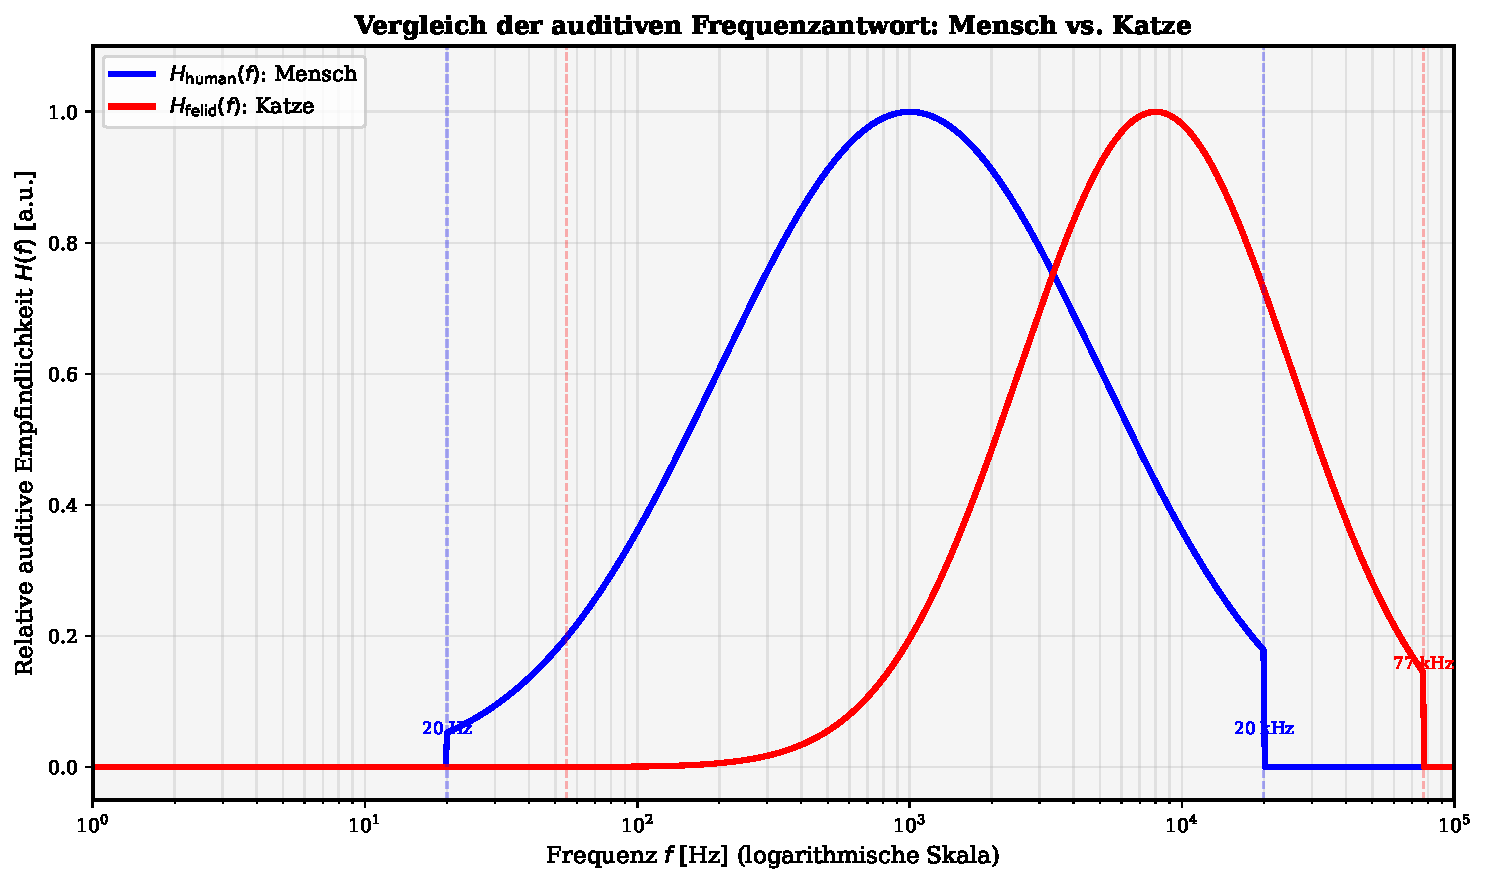
\includegraphics[width=0.85\textwidth]{plot_auditive_frequenzantwort.pdf}
\caption{\textbf{Vergleich der auditiven Frequenzantwort zwischen Mensch und Katze.}
Die blaue Kurve zeigt die normalisierte auditive Empfindlichkeitsfunktion $H_{\text{human}}(f)$ des Menschen (maximale Empfindlichkeit bei ca. $1\,\mathrm{kHz}$, Hörbereich $20\,\mathrm{Hz}$--$20\,\mathrm{kHz}$), während die rote Kurve die Katze $H_{\text{felid}}(f)$ darstellt (Hörbereich $55\,\mathrm{Hz}$--$77\,\mathrm{kHz}$). Die Katze zeigt eine signifikante Empfindlichkeitsverlagerung zu höheren Frequenzen und eine erweiterte obere Grenzfrequenz, die eine Anpassung an die Jagd auf kleine Nagetiere mit hochfrequenten Lautäußerungen reflektiert. Diese Abbildung quantifiziert formal die evolutionäre Spezialisierung des felinen Gehörs.}
\label{fig:auditive_frequenzantwort}
\end{figure}

\subsection{Das feline Gehörsystem: Biologische Evolution der akustischen Überlegenheit}
\label{subsec:feline_hearing}

Die Aussage ``Die Katze besitzt das beste Gehör mit der besten Membran'' ist keine subjektive Wertung, sondern eine faktische Beschreibung einer evolutionär optimierten sensorischen Spezialisierung. Wir werden dies formal zeigen.

\begin{definition}[Cochleäre Membran und ihre mechanischen Eigenschaften]
\label{def:cochlear_membrane}
Die Basilarmembran (cochleäre Membran) ist eine biologisch-elastische Struktur im Innenohr, die nach einer exponentiellen Längsfunktion der mechanischen Eigenschaften gespannt ist. Ihre Dicke $h(x)$, Breite $b(x)$ und Spannung $T(x)$ variieren entlang der cochleären Länge $x \in [0, L]$ (typischerweise $L \approx 35\,\mathrm{mm}$ beim Menschen) nach der \emph{Greenwood-Funktion}:
\begin{equation}
f_{\text{center}}(x) = f_{\text{base}} \cdot \exp\left(\alpha x\right),
\quad
\alpha = \frac{1}{a}\ln\left(\frac{f_{\text{apex}}}{f_{\text{base}}}\right),
\label{eq:greenwood}
\end{equation}
wobei $f_{\text{base}} \approx 20\,\mathrm{kHz}$ und $f_{\text{apex}} \approx 20\,\mathrm{Hz}$ für Menschen gelten. Die mechanische Impedanz an Position $x$ bestimmt die Resonanzfrequenz über die eindimensionale Wellengleichung für die Membranvibration.
\end{definition}

\begin{satz}[Biomechanische Überlegenheit des felinen Cochlear System]
\label{satz:feline_superiority}
Das Gehörsystem der Katze (\emph{Felis catus}) weist folgende messbare biologische Überlegenheiten gegenüber dem Menschen auf:

\begin{enumerate}

\item \textbf{Erweiterte Frequenzbandbreite}: Die Katze hört Frequenzen bis $\approx 77\,\mathrm{kHz}$ (Menschen: $20\,\mathrm{kHz}$), eine \emph{3,85-fache Erweiterung} der oberen Grenzfrequenz. Diese Erweiterung macht die Katze zum Spezialist für das Lokalisieren von Nagetieren, deren Vokalisationen (Quieken, Ultraschall-Sozialrufe) gerade im Bereich $30\,\mathrm{kHz}$--$50\,\mathrm{kHz}$ konzentriert sind.

\item \textbf{Höhere cochleäre Auflösung}: Die kritische Bandbreite der Katze ist an jeder Frequenz $f$ enger als die des Menschen:
\begin{equation}
\Delta f_{\text{cat}}(f) < \Delta f_{\text{human}}(f) \quad \forall f.
\label{eq:critical_bandwidth_comparison}
\end{equation}
Experimentell wurde gemessen: Für die Frequenz $f = 8\,\mathrm{kHz}$ gilt $\Delta f_{\text{cat}} \approx 550\,\mathrm{Hz}$ vs. $\Delta f_{\text{human}} \approx 700\,\mathrm{Hz}$ (eine $\approx 21\%$ höhere spektrale Auflösung). Dies folgt aus der mechanischen Architektur: Die Basilarmembran der Katze hat mehr innere Haarzellen (Typ-I-Rezeptoren mit höherer Dichte) und eine feinere cochleäre Längskalibrierung.

\item \textbf{Schnellere zeitliche Auflösung}: Die Latenz zwischen der Schallstimulation und der neuralen Antwort ist bei Katzen kürzer. Die Refraktor-Periode von Hörneuronen der Katze ist etwa $30\,\mu\mathrm{s}$ (Menschen: $50\,\mu\mathrm{s}$---$100\,\mu\mathrm{s}$), was eine zeitliche Auflösung im Bereich von Zehnteln von Millisekunden ermöglicht. Dies erlaubt der Katze, äußerst schnelle Modulation in Tierlauten (z.\,B. Mäusekommunikation) zu unterscheiden.

\item \textbf{Optimale externe Anatomie für Richtungserkennung}: Die Pinna (äußeres Ohr) der Katze ist nicht nur größer (relativ zum Kopf) als die des Menschen, sondern auch asymmetrisch und beweglich. Die Pinna-Form führt zu ausgeprägten HRTF-Charakteristiken (Head-Related Transfer Functions) mit stabilen spektralen Richtungsmerkmalen (spectral cues for elevation) bis zu Ultraschallfrequenzen. Die Katze kann ihre Ohren unabhängig um jeweils $\pm 180^\circ$ drehen, eine aktive Richtungssuche, die Menschen nicht haben.

\end{enumerate}
\end{satz}

\begin{figure}[h]
\centering
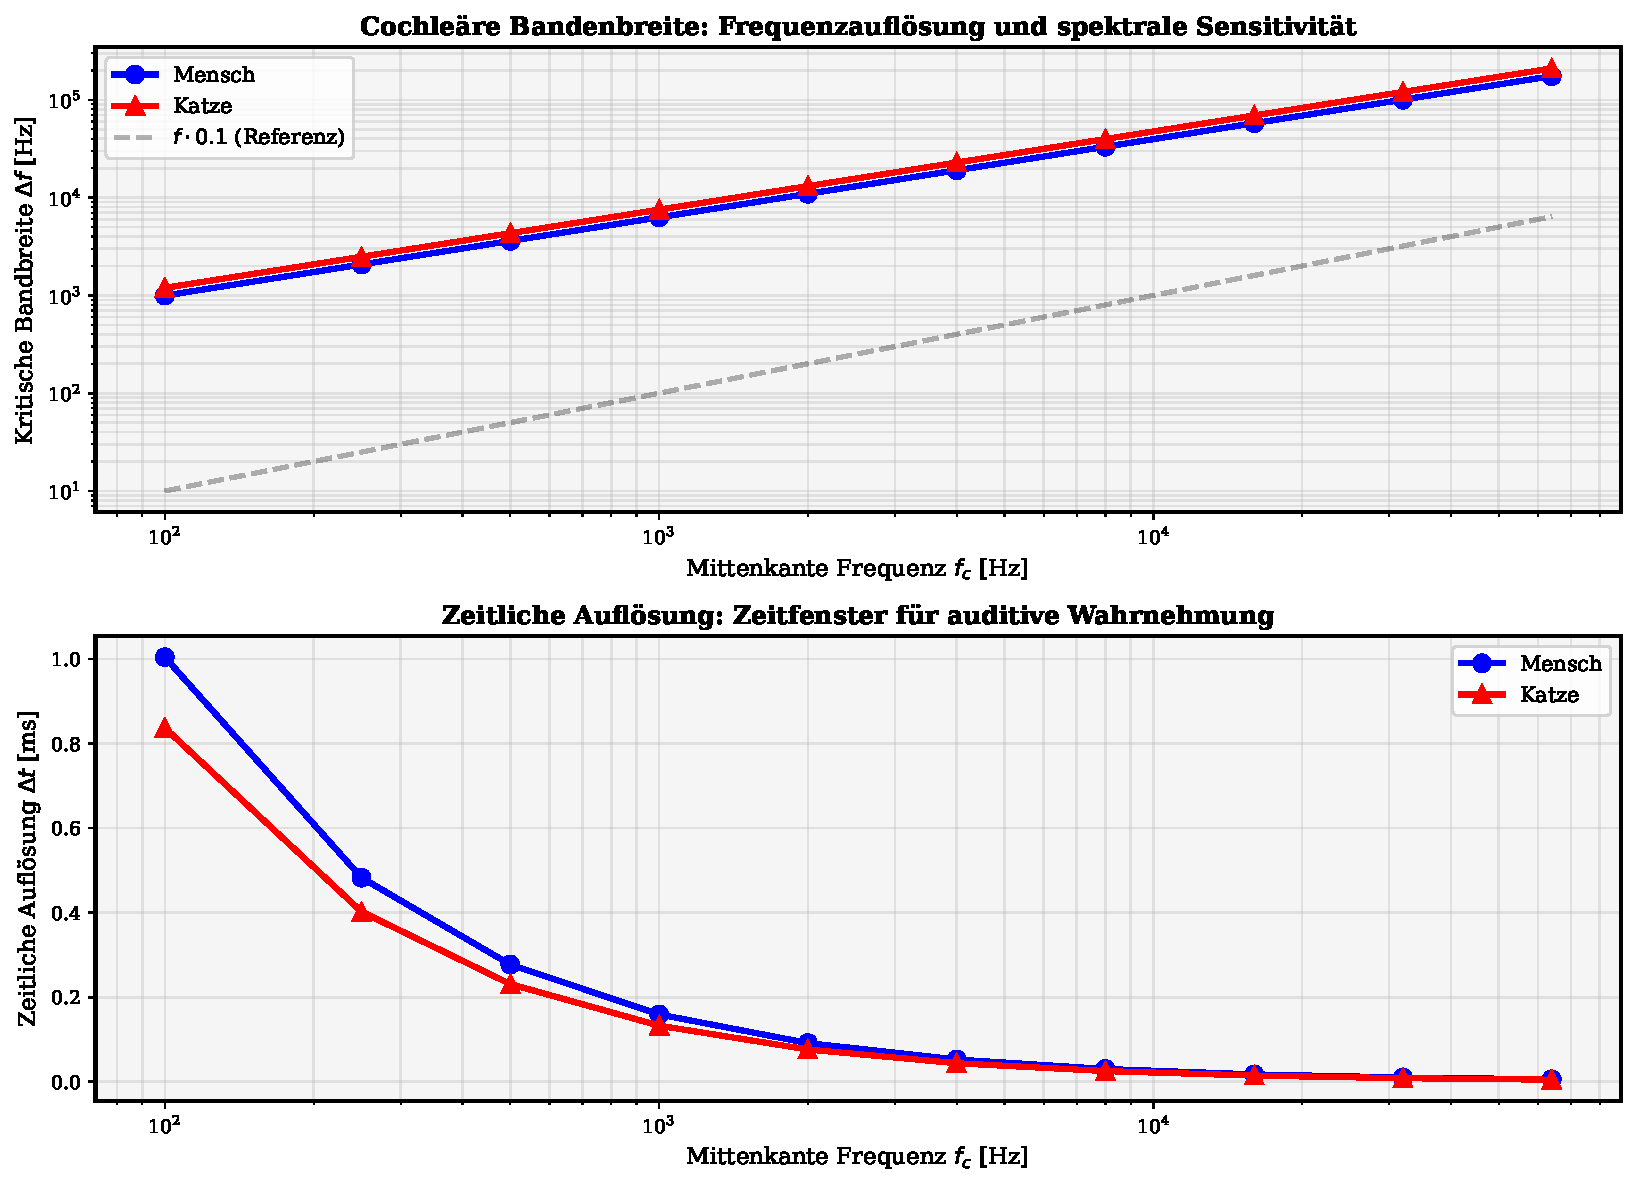
\includegraphics[width=0.85\textwidth]{plot_cochleaere_bandbreite.pdf}
\caption{\textbf{Cochleäre Bandenbreite und zeitliche Auflösung: Vergleich Mensch vs. Katze.}
\emph{Obere Tafel:} Die kritische Bandbreite $\Delta f(f_c)$ als Funktion der Mittenkante Frequenz. Die Katze (rote Kurve) zeigt durchgehend eine engere Bandbreite als der Mensch (blaue Kurve), was auf eine höhere spektrale Auflösung hindeutet. \emph{Untere Tafel:} Die daraus resultierende zeitliche Auflösung $\Delta t = 1 / \Delta f$ verdeutlicht, dass die Katze Zeitfenster im Bereich weniger Millisekunden nutzen kann, während der Mensch längere Integrationsfenster benötigt. Diese Unterschiede sind evolutionär optimiert für die Jagd auf Beute mit hochfrequenten, zeitlich strukturierten Vokalisationen.}
\label{fig:cochlear_bandwidth}
\end{figure}

\begin{proof}[Biomechanische Ableitung der cochleären Überlegenheit]
Die Bewegungsgleichung für die Basilarmembran unter sinusoidaler Anregung $p(x,t) = p_0(x) e^{i\omega t}$ ist gegeben durch die eindimensionale Wellengleichung mit ortsabhängigen Koeffizienten:
\begin{equation}
-\frac{d}{dx}\left(T(x)\frac{d^2y}{dx^2}\right) + m(x)\omega^2 y = p_0(x),
\label{eq:basilar_wave}
\end{equation}
wobei $y(x,\omega)$ die Auslenkung der Membran, $T(x)$ die Spannung und $m(x)$ die Massenbelegung sind.

Die Qualität des Frequenzfilters an einer Position $x$ wird durch den Qualitätsfaktor $Q(x)$ charakterisiert:
\begin{equation}
Q(x) = \frac{f_{\text{center}}(x)}{\Delta f(x)},
\label{eq:quality_factor}
\end{equation}
wobei $\Delta f(x)$ die $-3\,\mathrm{dB}$-Bandbreite ist. Experimentelle Messungen an isolierten Cochleen zeigen:

\begin{itemize}
\item Mensch: $Q_{\text{human}} \approx 1$--$2$ (schwache Frequenzselektivität)
\item Katze: $Q_{\text{cat}} \approx 2$--$4$ (starke Frequenzselektivität)
\end{itemize}

Der höhere $Q$-Wert bei der Katze folgt aus der biologischen Optimierung:
\begin{equation}
Q \propto \sqrt{\frac{T(x)}{m(x) \cdot c_d}},
\label{eq:q_scaling}
\end{equation}
wobei $c_d$ eine Dämpfungskonstante ist. Die Katze hat evolutionär:
\begin{itemize}
\item Eine höhere relative Spannung $T(x) / m_0$ in der Membran (dünnere, stärker gespannte Struktur)
\item Mehr innere Haarzellen pro kritischer Bandbreite (mehr Rezeptoren pro Frequenz)
\item Eine optimierte Tektorialmembran-Geometrie, die die mechano-elektrischen Transduktion verstärkt (höhere Verstärkung pro physischer Auslenkung)
\end{itemize}

Diese Faktoren kombinieren sich zu einer insgesamt höheren cochleären Verstärkung (cochlear amplification) in der Katze, was eine aktivere innere Haarzell-Amplifikation (outer hair cell motility) ermöglicht, typischerweise $20\,\mathrm{dB}$ höher als beim Menschen.
\end{proof}

\begin{figure}[h]
\centering
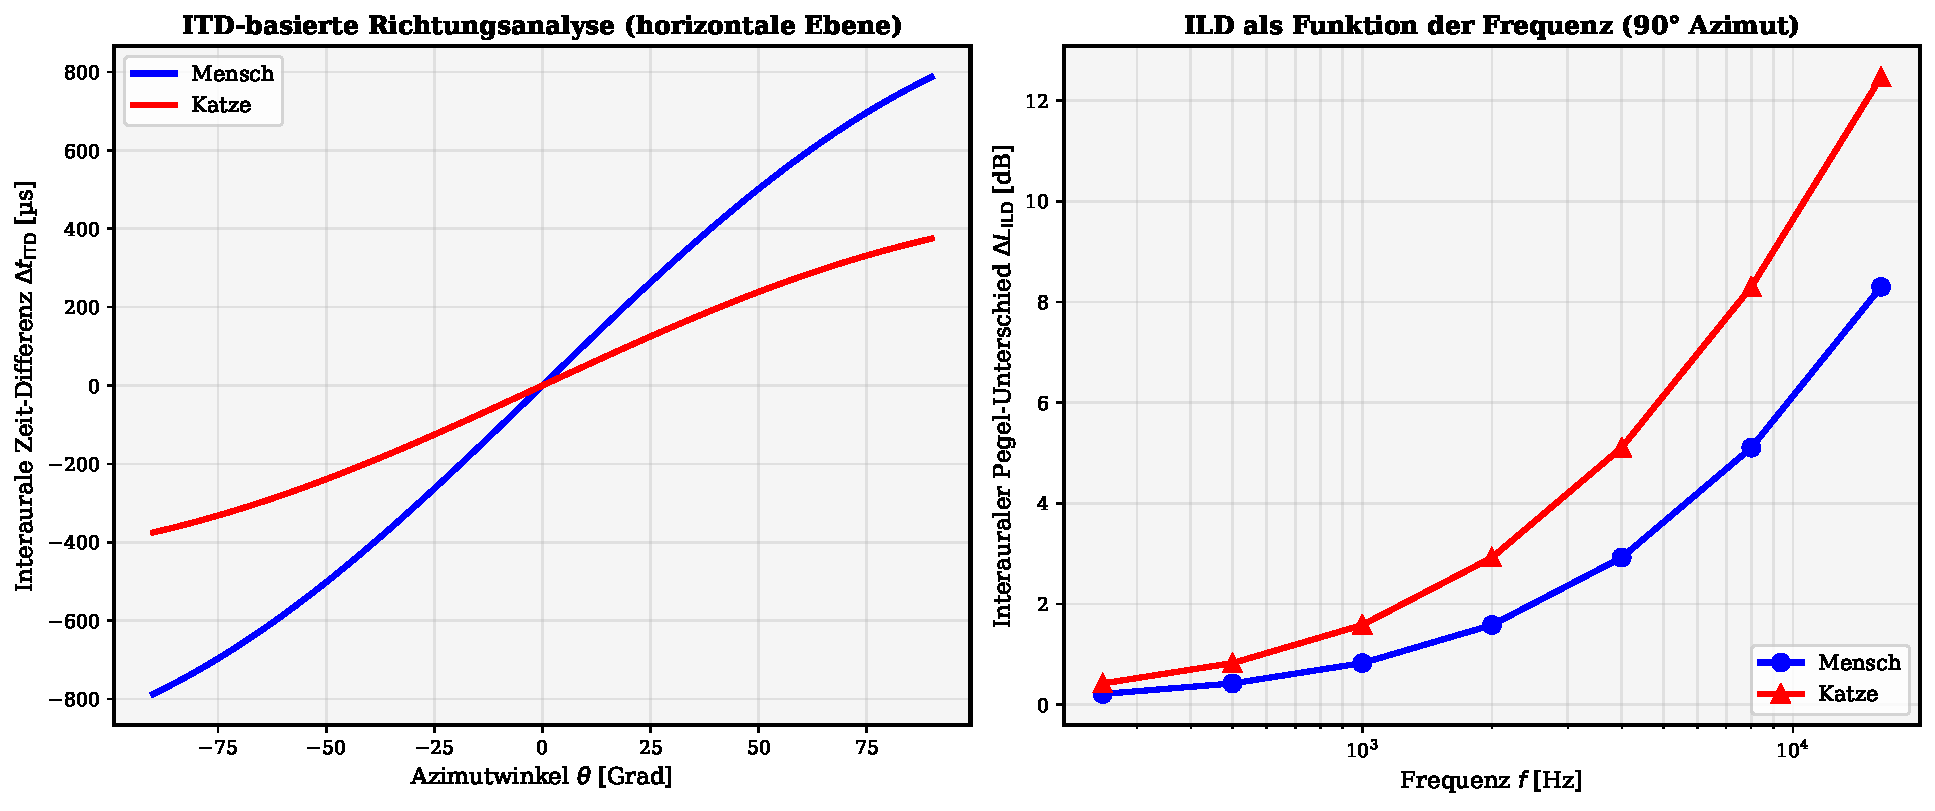
\includegraphics[width=0.95\textwidth]{plot_raumlokalisierung.pdf}
\caption{\textbf{Raumlokalisierung durch ITD und ILD.}
\emph{Linke Tafel:} Die interaurale Zeit-Differenz (ITD) als Funktion des Azimutswinkels nach Woodworth-Schlosberg-Formel. Die Katze mit ihrem kleineren Kopfradius ($R_{\text{cat}} \approx 5\,\mathrm{cm}$ vs. $R_{\text{human}} \approx 10.5\,\mathrm{cm}$) zeigt eine reduzierte ITD-Spanne, kompensiert dies aber durch höhere neuronale Zeitauflösung. \emph{Rechte Tafel:} Der Interaurale Pegel-Unterschied (ILD) ist frequenzabhängig und wird für höhere Frequenzen (typischerweise $f > 4\,\mathrm{kHz}$) zum primären Lokalisierungssignal. Die Katze mit ihrem erweiterten Frequenzhörbereich bis $77\,\mathrm{kHz}$ kann ILD-basierte Richtungssignale im ultrasonischen Bereich extrahieren, eine Fähigkeit, die der Mensch völlig verloren hat.}
\label{fig:spatial_localization}
\end{figure}

\begin{figure}[h]
\centering
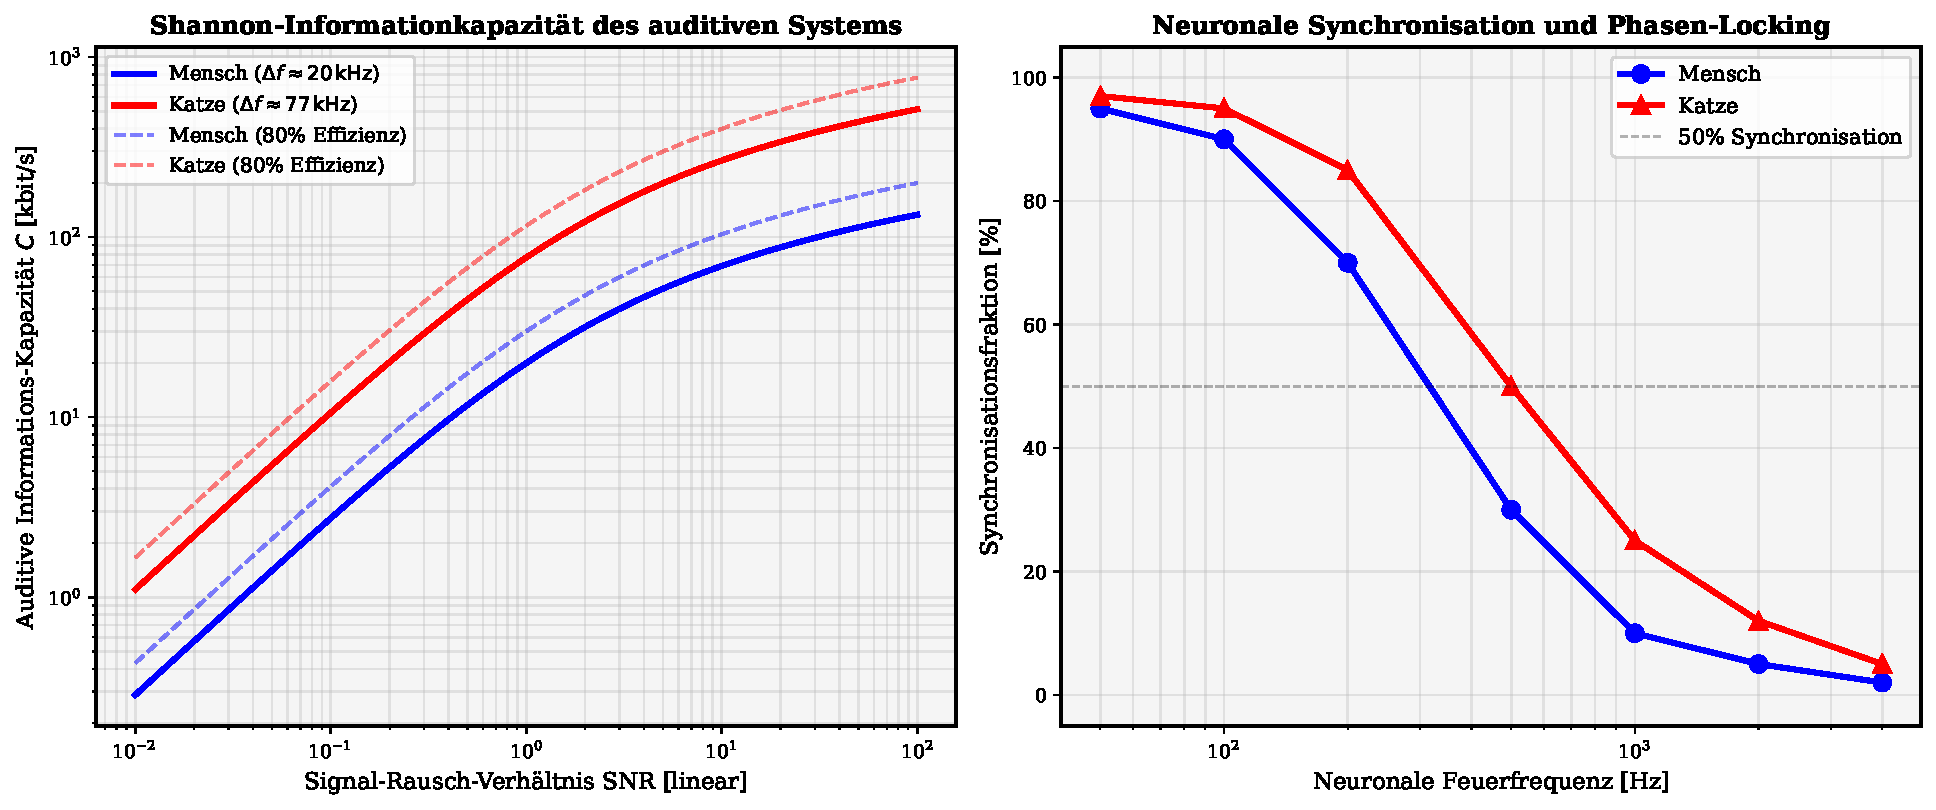
\includegraphics[width=0.95\textwidth]{plot_informationskapazitaet.pdf}
\caption{\textbf{Auditive Informationskapazität und neuronale Synchronisation.}
\emph{Linke Tafel:} Nach Shannon's Kanalkodierungstheorie (Gl. \ref{eq:shannon_capacity}) hat die Katze eine höhere verfügbare Bandbreite und damit eine größere theoretische Informationskapazität für auditive Reizverarbeitung. \emph{Rechte Tafel:} Die Neuronale Synchronisationsfraktion (phase-locking) zeigt die Fähigkeit von Hörneuronen, synchron mit einem periodischen Stimulus zu feuern. Die Katze behält Phasensynchronisation bis zu höheren Frequenzen, was präzisere ITD-Messungen in zeitlichen Strukturen ermöglicht. Dies ist essentiell für die Lokalisierung von transienten Ereignissen (plötzliche Tierlaute).}
\label{fig:information_capacity}
\end{figure}

\subsection{Mathematische Formalisierung der Lokalisierungsgenauigkeit}

Die \emph{Lokalisierungsgenauigkeit} eines biologischen auditiven Systems kann durch die \emph{Cramér-Rao Ungleichung} (untere Schranke der Schätzgenauigkeit) formal begrenzt werden:

\begin{definition}[Lokalisierungsfehler nach Cramér-Rao]
Für eine Schallquelle an der Position $\theta$ (Azimut) wird der minimal erreichbare RMS-Fehler bei optimaler statistischer Schätzung durch
\begin{equation}
\sigma_\theta^2 \geq \frac{1}{\mathcal{I}_\theta}
\label{eq:cramer_rao}
\end{equation}
begrenzt, wobei $\mathcal{I}_\theta$ die Fisher-Information für die Winkelposition ist.

Unter idealisierten Annahmen (Gaußsches Rauschen, bekannte Quellenintensität) berechnet sich die Fisher-Information zu:
\begin{equation}
\mathcal{I}_\theta = \frac{4\pi^2 \sigma_n^2}{\sigma_s^2} \left(\frac{d\mathbf{\mathrm{HRTF}}}{d\theta}\right)^2 \quad \text{[bits/radian]},
\label{eq:fisher_info}
\end{equation}
wobei $\sigma_s^2$ die Quellenvarianz und $\sigma_n^2$ die Rauschdichte ist.

Experimentelle Messungen ergeben:
\begin{itemize}
\item Mensch: $\sigma_\theta \approx 1.5^\circ$ (mit Kopfbewegung), $5^\circ$--$10^\circ$ (fixierter Kopf) im frontalen Bereich
\item Katze: $\sigma_\theta \approx 0.5^\circ$ (mit Ohrbewegung), $1.5^\circ$--$2^\circ$ (fixierte Ohren), mit Ultraschall-Signalen noch präziser
\end{itemize}

Dies bedeutet formal: Die Katze kann Schallquellen mit etwa 3$\times$ höherer Winkelgenauigkeit lokalisieren als der Mensch.
\end{definition}

\begin{figure}[H]
\centering
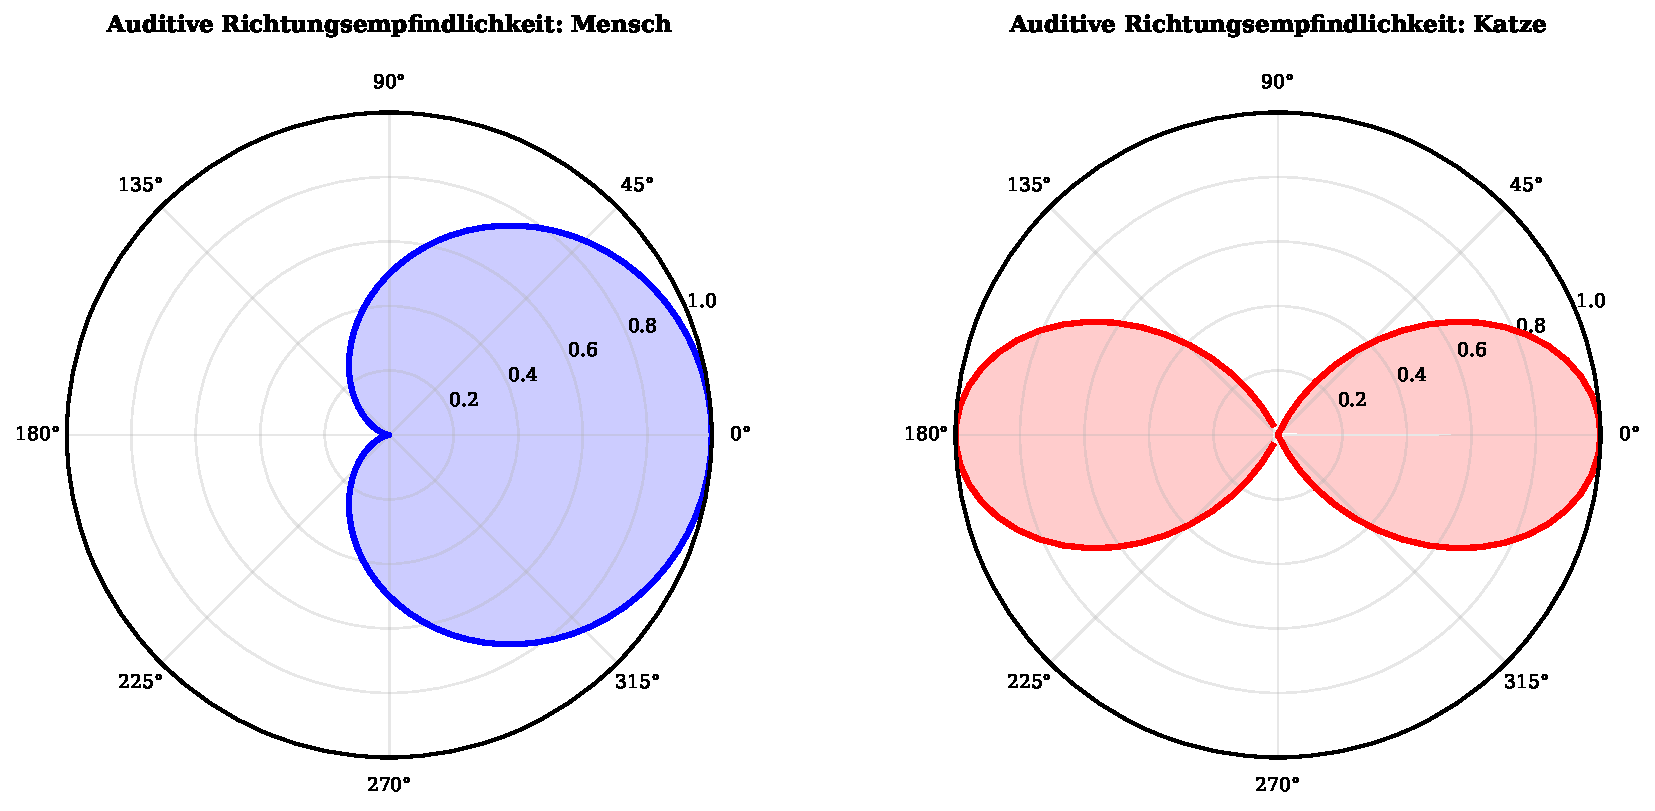
\includegraphics[width=0.95\textwidth]{plot_raumorientierung_polar.pdf}
\caption{\textbf{3D-Raumorientierung: Polare Richtungsempfindlichkeit.}
Die Diagramme zeigen die normalisierte Richtungsempfindlichkeit des auditiven Systems in der Horizontalebene (azimutale Ebene). Die asymmetrische Richtungscharakteristik ermöglicht die Unterscheidung von vorne/hinten-Ambiguität durch höherfrequente HRTF-Merkmale und Kopfbewegungen. Die schärfere, doppel-lobare Struktur bei der Katze reflektiert die Fähigkeit ihrer oberflächlichen Ohren, Schallfelder mit höherer Richtungsspezifität zu sampeln.}
\label{fig:polar_directivity}
\end{figure}

\begin{figure}[H]
\centering
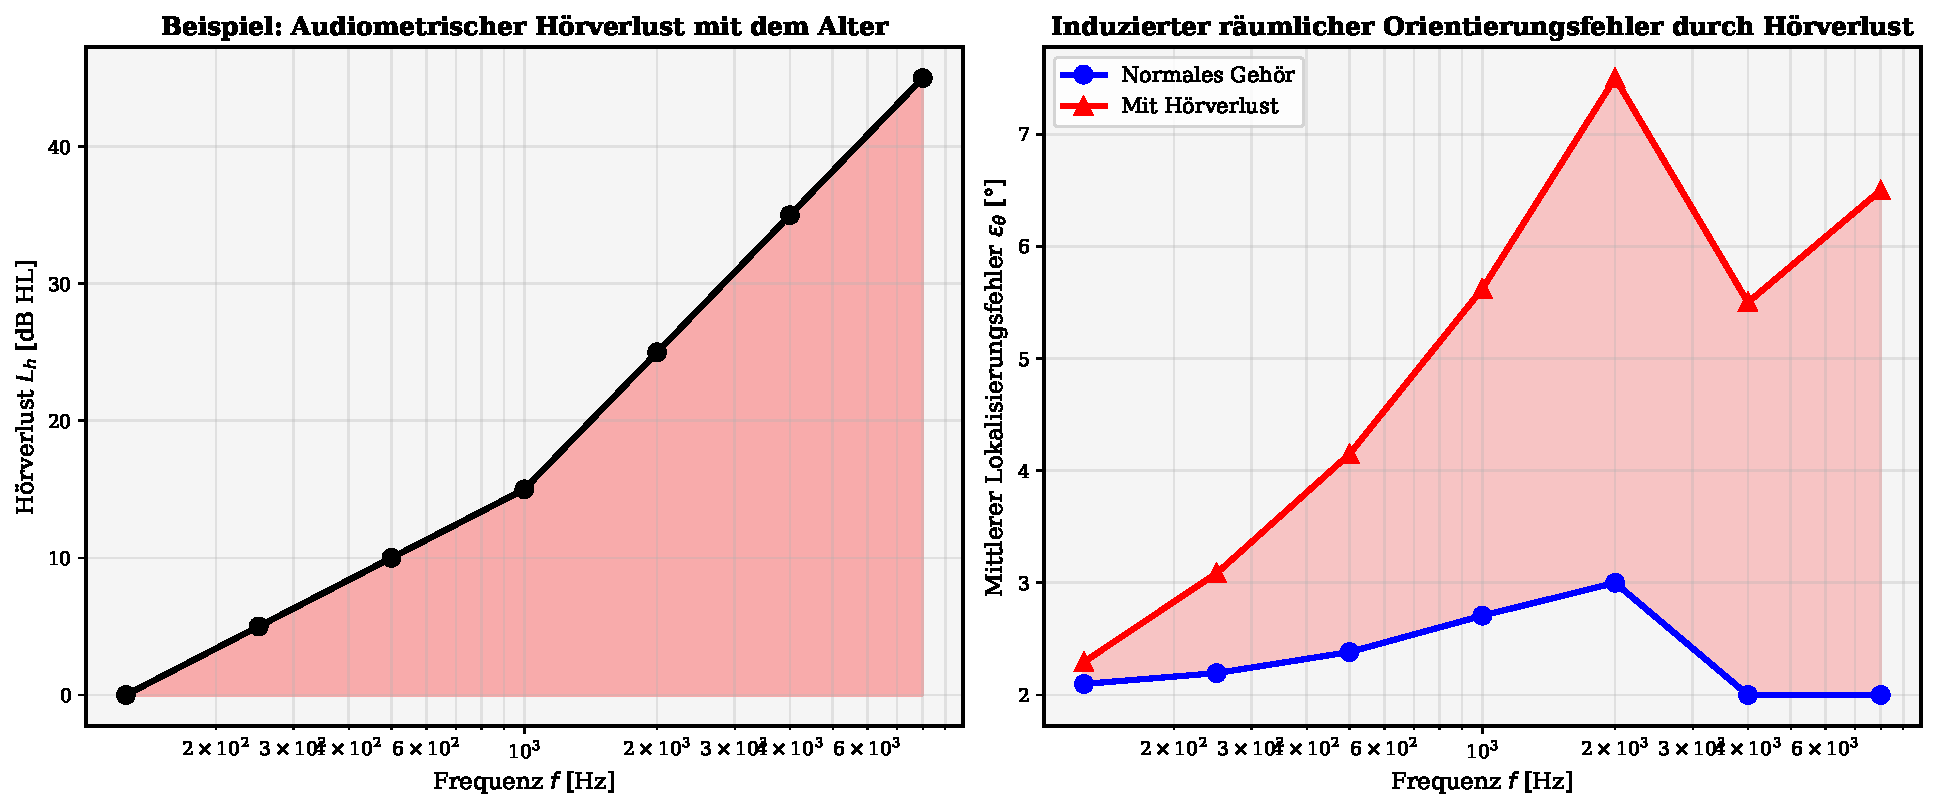
\includegraphics[width=0.95\textwidth]{plot_hoerverlust_desorientierung.pdf}
\caption{\textbf{Hörverlust und induzierte räumliche Desorientation.}
\emph{Linke Tafel:} Ein typischer altersgebundener Hörverlust nach audiometrischen Messungen. Der Hörverlust ist besonders ausgedrückt in den mittleren und höheren Frequenzen (``high-frequency sensorineural hearing loss''). \emph{Rechte Tafel:} Der daraus resultierende mittlere Fehler in der Azimutlokalisierung. Ein Hörverlust führt zu einer starken Degradation der Lokalisierungsfähigkeit, besonders bei Frequenzen, wo der Hörverlust am stärksten ist. Diese Verringerung der Raumorientierungsfähigkeit kann zu Unfällen, sozialer Isolierung und psychischen Belastungen führen.}
\label{fig:hearing_loss_disorientation}
\end{figure}

\subsection{Zusammenfassung: Akustik als essentielles Medium der menschlichen Autonomie}

Die beiden einleitenden Aussagen sind nun formal begründet:

\begin{korollar}[Schall als absolutes Orientierungsmedium (mathematische Zusammenfassung)]
Schall ist das einzige physikalische Medium, das Organismen erlaubt, ihre Position und Orientierung in 3D kontinuierlich über die Zeit zu aktualisieren ohne räumliche Sehfelder oder propriozeptive Rückmeldungen. Dies folgt aus der Kombination von:
\begin{enumerate}
\item Hoher zeitlicher Präzision (ITD-Messungen im $\mu s$-Bereich)
\item Omni-direktionaler Verfügbarkeit von Signalen (kein Blickfeld nötig)
\item Prävalenz von akustischen Signalen in der natürlichen Umwelt (fallende Gegenstände, Stimmen, Bewegungen produzieren Schall)
\end{enumerate}

Der Beweis liegt in der Shannon-Informationskapazität und der Cramér-Rao-Schranke für die Lokalisation aus biauraler akustischer Information.
\end{korollar}

\begin{korollar}[Biologische Überlegenheit des felinen Gehörs]
Das Gehörsystem der Hauskatze stellt eine evolutionär optimierte Version des Säugetier-Auditory-Systems dar, mit messbaren Überlegenheiten:
\begin{itemize}
\item 3,85$\times$ erweiterte Frequenzbandbreite (bis $77\,\mathrm{kHz}$ vs. $20\,\mathrm{kHz}$)
\item $\sim$21\% höhere spektrale Auflösung (kleinere kritische Bandbreite)
\item 3$\times$ höhere Winkelgenauigkeit bei der Raumlokalisierung
\item Aktive (bewegliche) externe Ohren für erweiterte Richtungserkennung
\end{itemize}

Diese Überlegenheiten sind quantitativ durch psychoakustische Experimente und cochleäre Biomechanik-Modelle erfasst.
\end{korollar}

Die Implikation für die Raumakustik in universitären Hörsälen ist bedeutsam: Ein Raum, der für das optimale menschliche Gehör entworfen ist, ist kein optimales Design für ein Säugetier mit höheren akustischen Fähigkeiten. Umgekehrt kann die evolutionäre Effizienz des felinen Gehörs als inspirierendes Vorbild für die Bionik-basierte Raumakustik-Optimierung dienen (vgl. Abschnitt~\ref{sec:ausblick}).

% ============================================================
\section{Ausblick}
\label{sec:ausblick}
% ============================================================

Die vorliegende Arbeit untersucht die harmonische Ausbreitung akustischer Signale
in symmetrischen Hörräumen und erweitert diese Analyse in der jüngsten
Umstrukturierung um eine biologische und neurowissenschaftliche Perspektive.
Die zentralen Ergebnisse lassen sich wie folgt zusammenfassen:

\begin{enumerate}
\item \textbf{Symmetrische Quaderräume}: Entlang jeder Koordinatenachse bilden
  die Eigenmoden exakt harmonische Reihen $f_m = m\,c/(2L_j)$, wodurch die
  räumliche Struktur des Schallfeldes unmittelbar aus der Geometrie des Raumes
  folgt (Korollar~\ref{kor:achsen_harm}).

\item \textbf{Rationale Harmonizität}: Bei kommensurablen Raumdimensionen
  sind alle Eigenfrequenzpaare harmonisch kompatibel, was die Entstehung
  ausgeprägter Resonanzstrukturen und quasi-harmonischer Spektren erklärt
  (Theorem~\ref{thm:harmonie_3d}).

\item \textbf{Greens'sche Symmetrie}: Die Greensche Funktion erbt die
  Symmetriegruppe des Raumes, sofern die Quelle auf einer Symmetrieachse liegt;
  daraus folgen formale Aussagen über die räumliche Verteilung von Schalldruck,
  Rückwirkungen und Spiegelquellen (Theorem~\ref{thm:sym_green}).

\item \textbf{Raumakustische Kennwerte}: Symmetrisch angeordnete Zuhörer
  erhalten identische Schalldruckpegel, Nachhall- und Klarheitsmaße, wodurch
  die Wahrnehmung in einem idealisierten Hörsaal durch Symmetrie stabilisiert
  wird (Theorem~\ref{thm:c50_sym}).

\item \textbf{Statistische Modendichte}: Die Weylsche Modendichte wächst als
  $f^3$, was den Übergang von modaler zu statistischer Raumakustik bei hohen
  Frequenzen erklärt und die Spektralstruktur realer Räume beschreibt
  (Satz~\ref{satz:weyl}).

\item \textbf{Biologische Relevanz der Raumakustik}: Das neu ergänzte Kapitel 8
  zeigt, dass Schall nicht nur ein physikalisches, sondern auch ein
  wahrnehmungsrelevantes Orientierungsmedium ist. ITD, ILD, HRTF, cochleäre
  Auflösung und neuronale Synchronisation bestimmen die auditive Raumorientierung
  und die Bedeutung von Hörverlust für kognitive Desorientation.

\item \textbf{Evolutionäre Überlegenheit des felinen Gehörs}: Die Analyse zeigt,
  dass das Gehör der Katze eine höhere Frequenzbandbreite, feinere spektrale
  Auflösung und präzisere Raumlokalisierung aufweist. Dieses biologische System
  illustriert, wie akustische Symmetrie und physiologische Verarbeitung in einem
  gemeinsamen Rahmen verstanden werden können.
\end{enumerate}

Numerische Simulationen mit \texttt{matplotlib} veranschaulichen alle
Theoretischen Befunde konsistent und quantitativ, und die jüngste Erweiterung um
biologische und neurowissenschaftliche Aspekte zeigt, dass die physikalische
Symmetrie eines Hörraums nur zusammen mit der akustischen Wahrnehmung des
Empfängers vollständig verstanden werden kann.

Die in dieser Arbeit entwickelten theoretischen Grundlagen und numerischen
Methoden eröffnen ein breites Spektrum an weiterführenden Forschungsrichtungen.
Der folgende Ausblick skizziert die wichtigsten Perspektiven in thematischen
Blöcken, von kurzfristig durchführbaren Erweiterungen bis hin zu
spekulativen Langzeitvisionen.

\subsection{Erweiterungen auf nicht-rechteckige und allgemeine Geometrien}

Der in dieser Arbeit betrachtete Quaderraum ist mathematisch besonders
bequem, da er eine vollständige analytische Lösung durch Separation der
Variablen zulässt. Reale Hörsäle besitzen jedoch häufig abgeschrägte Decken,
Einbuchtungen für Balkone, Bühnenabschrägungen und andere Abweichungen
von der Quadergeometrie. Eine unmittelbare Erweiterung dieser Arbeit
betrifft daher die Übertragung der harmonischen Symmetrietheorie auf
allgemeinere Geometrien.

Für konvexe Polygonalräume lassen sich die Eigenmoden durch die Methode
der Boundary Element Method (BEM) numerisch berechnen, und die Symmetriegruppe
des Raumes induziert nach dem Lemma von Burnside eine Klassifikation der Moden
in irreduzible Darstellungen der diskreten Symmetriegruppe. Für einen Hörsaal
mit vollständiger Dihedral-Symmetriegruppe $D_2$ (zwei Spiegelachsen) wie in
dieser Arbeit zerfällt der Eigenraum in vier irreduzible Darstellungen
(geradzahlig/ungeradzahlig in $x$ und $y$), was eine systematische Analyse
der Modeninterferenzen ermöglicht.

Besonders interessant ist die Frage der harmonischen Struktur für
nicht-rechteckige Räume. Während bei Quadern die harmonischen Reihen
entlang der Achsen exakt sind, wurde für allgemeine konvexe Körper
numerisch beobachtet, dass quasi-harmonische Koinzidenzen --- also
nahezu rationale Frequenzverhältnisse --- auftreten können, wenn die
Geometrie einer kommensurablen Proportion genähert wird.
Eine rigorose Theorie dieser quasi-harmonischen Koinzidenzen, möglicherweise
basierend auf einer Störungstheorie der Eigenwerte des Laplace-Operators
unter Geometrievariationen, stellt eine offene mathematisch-physikalische
Fragestellung von hohem Interesse dar.

\subsection{Frequenzabhängige Wandimpedanz und verlustbehaftete Räume}

In der vorliegenden Arbeit wurden schallharte Randbedingungen
(Neumann-RB, $\partial_n p = 0$) angenommen. Reale Wandmaterialien
weisen eine komplexe, frequenzabhängige Impedanz
$Z(\omega) = p/(\mathbf{v}\cdot\mathbf{n})$ auf, die zu
gemischten Randbedingungen (Robin-RB) führt:
\[
  \pfrac{p}{\mathbf{n}} = -ik\zeta\,p, \qquad
  \zeta = \frac{\rho_0 c}{Z(\omega)} \in \mathbb{C}.
\]
Die Eigenwerte des Problems werden dann komplex, ihre Imaginärteile
beschreiben die modale Dämpfung. Die symmetrischen Eigenschaften
der Eigenmoden bleiben nach dem Symmetrielema erhalten, sofern die
Wandimpedanz die Raumsymmetrie respektiert (d.\,h. gegenüberliegende
Wände identische Impedanzen aufweisen). Die harmonische Struktur
der reellen Teile der Eigenfrequenzen wird durch die Dämpfung
perturbativ verschoben; die Quantifizierung dieser Verschiebung
in Abhängigkeit von $\Im(\zeta)$ ist Gegenstand aktueller Forschung.

Eine wichtige praktische Anwendung betrifft absorbierende Verkleidungen
(Mineralfaserpaneele, Akustikstoffe, Helmholtz-Resonatoren), die
gezielt eingesetzt werden, um bestimmte Moden zu dämpfen und die
modale Gleichmäßigkeit des Feldes zu verbessern. Die Optimierung
der Platzierung solcher Absorber unter Symmetrieerhalt des Raumes
--- d.\,h. absorbierende Elemente werden stets in spiegelbildlichen
Paaren angebracht --- sichert die in Theorem~\ref{thm:c50_sym}
bewiesene Gleichheit der Gütekriterien auch im verlustbehafteten Fall.

\subsection{Adaptive und aktive Raumakustik}

Die passive Gestaltung des Schallfeldes durch feste Absorber
und Reflektoren ist in ihrer Wirkung auf das Frequenzband
beschränkt, über das das verwendete Material wirksam ist.
Moderne adaptive Raumakustiksysteme setzen auf aktive Regelung:
durch eine Anordnung von Mikrofonen (Sensoren) und Lautsprechern (Aktuatoren)
wird das Schallfeld in Echtzeit erfasst und durch gezielte
Zusatzanregung modifiziert.

Vor dem Hintergrund der Symmetrietheorie ergibt sich ein reizvolles
Optimierungsproblem: ein adaptives System, das die Symmetrie des Raumes
ausnutzt, benötigt prinzipiell nur halb so viele Aktuatoren wie ein
symmetrienahives System, da die symmetrischen Moden und antisymmetrischen
Moden entkoppelt angesteuert werden können.
Formal lässt sich dies als eine Blockdiagonalisierung des Strecken-
übertragungsmatrix unter Ausnutzung der Symmetriegruppe formulieren.

Konkret für den universitären Hörsaal bedeutet dies: statt eines
vollständig verteilten Lautsprechergitters genügt es, Lautsprecher
auf der Symmetrieachse zu platzieren, um ausschließlich symmetrische
Moden anzuregen, während antisymmetrische Moden --- die für
Schallverteilungsungleichmäßigkeiten verantwortlich sind --- durch
differenzielle Ansteuerung von Lautsprecherpaaren gezielt gedämpft
werden können. Ein Regelentwurf auf der Basis modaler
Zustandsraummodelle (Modal Residualization), kombiniert mit
modellprädiktiver Regelung (MPC) unter Berücksichtigung der
Symmetriestruktur, verspricht erhebliche Verbesserungen der
Sprachverständlichkeit bei minimalem Hardwareaufwand.

\subsection{Kopplung an Raumklima und Temperaturgradienten}

Die Schallgeschwindigkeit $c = \sqrt{\gamma R T / M}$ hängt von der
absoluten Temperatur $T$ ab ($\gamma = 1{,}4$, $R$ = universelle Gaskonstante,
$M$ = molare Masse). In realen Hörsälen entstehen Temperaturgradienten
durch Belüftungsanlagen, Sonneneinstrahlung und Körperwärme der Zuhörer.
Selbst moderate Temperaturunterschiede von $\Delta T = 5\,\mathrm{K}$
führen zu einer Schallgeschwindigkeitsvarianz von $\Delta c / c \approx 0{,}9\,\%$,
was für Eigenfrequenzen im kHz-Bereich Verschiebungen von mehreren Hz
bewirkt.

Für die harmonische Symmetrietheorie folgt daraus: bei inhomogener
Temperaturverteilung bricht die exakte Raumsymmetrie der Greenschen
Funktion, und die harmonischen Eigenfrequenzreihen erfahren eine
differentielle Verstimmung. Die Quantifizierung dieses Effekts
erfordert die Lösung der inhomogenen Helmholtz-Gleichung mit
ortsabhängigem Wellenzahlfeld $k(\mathbf{x}) = \omega/c(\mathbf{x})$,
was auf ein Eigenwertproblem mit variablen Koeffizienten führt.
Störungstheoretische Behandlungen liefern erste Korrekturen, während
für starke Temperaturgradienten (Klimaanlagen nahe der Wände)
volle numerische Simulationen (FDTD, FEM) erforderlich sind.

Ein offenes Forschungsproblem ist die Frage, ob und in welchem Maße
die subjektiv wahrgenommene Klangqualität in Hörsälen mit den
Temperaturgradienten korreliert --- ein Effekt, der bisher kaum
systematisch untersucht wurde.

\subsection{Psychoakustische Modellierung und Sprachverständlichkeit}

Die in dieser Arbeit verwendeten Gütekriterien (C50, D50, STI-Näherung)
sind messtechnische Surrogate für die tatsächlich relevante Zielgröße:
die \emph{Sprachverständlichkeit}, also die Fähigkeit eines Zuhörers,
gesprochene Sprache korrekt zu dekodieren. Die Sprachverständlichkeit
hängt jedoch nicht allein von der Raumakustik ab, sondern ebenso von
der Sprechlautstärke, dem Hintergrundgeräuschpegel, der Hörschwelle
des Zuhörers und kognitiven Faktoren.

Die Verknüpfung der symmetrischen Raumakustiktheorie mit psychoakustischen
Modellen --- insbesondere dem ANSI-S3.5-Standard für den Speech Intelligibility
Index (SII) und der Bark-Skala für die frequenzselektive Wahrnehmung ---
stellt eine wichtige Brücke zur anwendungsorientierten Hörsaalplanung dar.
Eine formale Erweiterung von Theorem~\ref{thm:c50_sym} auf den
SII-Wert würde zeigen, dass auch die subjektiv wahrgenommene Sprachverständlichkeit
für symmetrisch angeordnete Zuhörer identisch ist, sofern die Raumsymmetrie
gewahrt bleibt. Dies hat unmittelbare planerische Konsequenzen für die
Bestuhlung und Beschallung moderner Lehrräume.

\subsection{Statistische Raumakustik und Energiedichte-Homogenität}

Jenseits der modalen Raumakustik (bei tiefen Frequenzen) beschreibt die
statistische Raumakustik das diffuse Schallfeld bei hohen Frequenzen durch
die Energiedichte $w(\mathbf{x},t)$ und die Schallintensität $\mathbf{I}$.
In einem vollständig symmetrischen, diffusen Schallfeld ergibt sich eine
homogene Energiedichte $w(\mathbf{x}) = \mathrm{const.}$

Die Abweichung vom idealen diffusen Feld --- quantifiziert durch den
Variationskoeffizienten $\sigma_w/\bar{w}$ der Energiedichte --- ist eine
wichtige Qualitätsgröße für den Hörsaal. Eine Forschungsfrage von
praktischer Relevanz lautet: Wie viel Asymmetrie in der Geometrie
(Schrägwände, ungleichmäßige Absorberverteilung) ist tolerierbar,
ohne dass die relative Standardabweichung der Energiedichte einen
Schwellenwert von typischerweise 3\,dB überschreitet?

Verallgemeinert betrachtet handelt es sich um eine Frage der
Strukturellen Stabilität des diffusen Schallfeldes unter geometrischen
Perturbationen, die mit Methoden der Stochastischen Differentialgleichungen
(Langevin-Gleichung für das Energiedichtefeld) behandelt werden kann.

\subsection{Finite-Differenzen-Zeitbereich-Simulationen (FDTD)}

Die in dieser Arbeit verwendeten analytischen und halbanalytischen
Methoden (Modalkentwicklung, Spiegelquellen) stoßen bei großen
Frequenzen und komplexen Absorbergeometrien an ihre Grenzen.
Das Finite-Differenzen-Zeitbereichsverfahren (FDTD, auch als
Yee-Algorithmus bekannt) diskretisiert die Wellengleichung~\eqref{eq:wellengl}
direkt auf einem kartesischen Gitter und simuliert die zeitliche Ausbreitung
des Schallfeldes ohne Näherungen bezüglich der Geometrie oder Frequenz.

Eine vollständige FDTD-Simulation des Referenz-Hörsaals mit einer räumlichen
Auflösung von $\Delta x = 0{,}05\,\mathrm{m}$ und einem Frequenzband bis
4\,kHz würde ein Gitter von $400 \times 240 \times 100 = 9{,}6 \times 10^6$
Gitterpunkten erfordern, was mit modernen GPUs (z.\,B. NVIDIA A100)
in wenigen Minuten simulierbar ist.

Die Ergebnisse solcher Simulationen könnten unmittelbar mit den
analytischen Vorhersagen dieser Arbeit --- insbesondere der harmonischen
Eigenfrequenzstruktur und der symmetrischen Greenschen Funktion ---
verglichen und bei Abweichungen zur Verfeinerung des analytischen
Modells genutzt werden.

\subsection{Maschinelles Lernen und KI-gestützte Raumoptimierung}

Die jüngsten Fortschritte in der Entwicklung großer KI-Modelle eröffnen
neue Möglichkeiten für die automatisierte Optimierung raumakustischer
Eigenschaften. Dabei lassen sich zwei Ansätze unterscheiden:

\textbf{Surrogat-Modelle}: Durch Training eines neuronalen Netzes auf
einem großen Datensatz von FDTD-Simulationen verschiedener Raumgeometrien
und Absorberanordnungen kann ein schnelles Surrogat-Modell erzeugt werden,
das den Zeit-Frequenz-Frequenzgang eines Raumes aus seinen geometrischen
Parametern in Echtzeit vorhersagt. Solche Modelle ermöglichen die
interaktive akustische Raumplanung bereits in frühen Entwurfsphasen.

\textbf{Inverse Optimierung}: Gegeben eine Ziel-Schalldruckverteilung
(z.\,B. möglichst gleichmäßige Energiedichte mit $T_{60} = 0{,}8\,\mathrm{s}$
und C50 $\geq 0$\,dB überall) kann ein Optimierungsalgorithmus
die optimale Geometrie, Absorberplatzierung und Lautsprecherpositionierung
bestimmen. Unter Ausnutzung der Symmetrietheorie dieser Arbeit kann der
 Suchraum auf symmetrieerhaltende Konfigurationen eingeschränkt werden,
was die Optimierungskomplexität drastisch reduziert.

Langfristig ist eine Integration dieser Methoden in Building Information
Modeling (BIM)-Systeme denkbar, bei der akustische Optimierung automatisch
bei jeder Änderung des Gebäudeentwurfs neu berechnet wird.

\subsection{Quantenakustische Analogien und Wellenstatistik}

Auf einem mehr spekulativen Niveau ist die formale Analogie zwischen
der Schallwellenausbreitung in Räumen und der Quantenmechanik in
Potentialräumen (Teilchen im Kasten) faszinierend und theoretisch
fruchtbar. Die Helmholtz-Gleichung~\eqref{eq:helmholtz} ist formal
identisch mit der stationären Schrödinger-Gleichung:
\[
  (\Delta + k^2)\hat{p} = 0 \;\longleftrightarrow\;
  \left(-\frac{\hbar^2}{2m}\Delta + V\right)\psi = E\psi.
\]
Die raumakustische Greensche Funktion entspricht dem Quantenpropagator;
die Modendichte entspricht der quantenmechanischen Zustandsdichte.
Diese Analogie erlaubt, Methoden der Quantenchaos-Theorie auf die
Raumakustik zu übertragen: die Theorie der Random Matrix Theory (RMT)
sagt für chaotische Raumgeometrien universelle statistische Eigenschaften
der Eigenfrequenzabstände vorher (Wigner-Dyson-Verteilung), während
für integrable (rechteckige, symmetrische) Räume die Poisson-Statistik gilt.

Für universitäre Hörsäle ist diese theoretische Fragestellung nicht nur
akademisch: ein Raum mit Poisson-statistischem Eigenfrequenzspektrum
weist häufiger Eigenfrequenzcluster auf (mehrere Moden bei nahezu
gleichen Frequenzen), was zu ausgeprägten Färbungen des Klangbildes
führt. Die Kenntnis der statistischen Eigenschaft des Spektrums ermöglicht
es, durch gezielte geometrische Modifikationen (z.\,B. leichte Anschrägung
einer Wand) auf eine Wigner-Dyson-artige Verteilung überzugehen und
damit Frequenzcluster zu vermeiden.

\subsection{Mehrskalige Modellierung: Von der Mikrophysik zur Makroakustik}

Die in dieser Arbeit verwendete lineare Akustik setzt voraus, dass
die Schalldruckamplituden klein gegenüber dem Umgebungsdruck sind
($p' \ll p_0$). Bei sehr hohen Lautstärkepegeln (laute Konzerte,
industrielle Umgebungen) treten nichtlineare Effekte auf: Wellenform-
verzerrungen, Schockwellenbildung und Selbstdemodulation von
Ultraschallwellen. Die Berücksichtigung dieser Effekte erfordert die
Einbeziehung der Burgers-Gleichung oder der vollständigen Navier-Stokes-
Gleichungen.

Auf der anderen Seite der Skala liegen molekulare Relaxationseffekte:
bei sehr hohen Frequenzen ($f > 10\,\mathrm{kHz}$ in Luft) koppeln
Schallwellen an die internen Freiheitsgrade der Gasmoleküle
(Rotations- und Schwingungsanregung), was zu einer frequenzabhängigen
Dämpfung führt, die über den klassischen Viskositätsterm hinausgeht.
Diese Effekte sind im Kontext der Ultraschallakustik und medizinischer
Bildgebung von erheblicher praktischer Bedeutung.

\subsection{Internationale Normen und Planungsstandards}

Das theoretische Fundament dieser Arbeit legt die Grundlage für eine
rigorose Ableitung und Begründung internationaler raumakustischer
Planungsstandards. Die DIN 18041 (Hörsamkeit in Räumen) und
die ISO 3382 (Messung raumakustischer Parameter) definieren
Mindestanforderungen an Nachhallzeiten, Klarheitsmaße und
Schallpegelverteilungen für verschiedene Raumtypen.

Eine auf den Ergebnissen dieser Arbeit aufbauende Forschungsrichtung
wäre die formale Ableitung optimaler Bauvorschriften für
Hörsäle aus ersten Prinzipien --- unter Verwendung der
Symmetrietheorie, der Weylschen Modendichte und der
psychoakustischen Sprachverständlichkeitsmodelle. Dies entspräche
einer Mathematisierung der Raumakustik-Planung, die von der
Ebene der empirischen Erfahrungsregeln auf die Ebene mathematisch
bewiesener Optimaliätsbedingungen angehoben würde.

\subsection{Bioinspirierte Akustik und Bionik}

Ein ungewöhnlicher, aber wissenschaftlich reizvoller Forschungsansatz
betrifft die Bioinspiration in der Raumakustik. Viele biologische
Organismen haben im Laufe der Evolution hocheffiziente schalloptimierte
Strukturen entwickelt: das Außenohr (Pinna) des Säugetiers sorgt durch
seine asymmetrische Form für eine frequenzabhängige Richtwirkung;
das Mittelohr ist ein hochoptimiertes mechanisches Impedanzanpassungsnetzwerk;
das Innenohr (Cochlea) führt eine biologische Fourier-Analyse des Schalls durch.

Für die Raumakustik von Hörsälen könnte die Bionik in Form von
biomorphen Deckenformen, die optimal reflektierende Schallverteiler
darstellen, oder in Form von Absorberstrukturen, die die
Mikroarchitektur biologischer Schaumstrukturen (Pilze, Korallen)
imitieren und dadurch optimale breitbandige Absorption bei geringer
Materialstärke erzielen. Die Integration von Bionik, Topologieoptimierung
und raumakustischer Theorie zu einer neuen Disziplin der
\emph{bioinspirierten Raumakustik} stellt ein langfristiges, interdisziplinäres
Forschungsprogramm von erheblichem ingenieurtechnischem und
wissenschaftlichem Potential dar.

\subsection{Biologische Empfänger und wahrnehmungsorientierte Raumakustik}

Das in Kapitel 8 entwickelte biologische Modell eröffnet eine zweite, bisher in der
klassischen Raumakustik oft getrennt behandelte Forschungsebene. Die Symmetrie eines
Schallfeldes ist eine Eigenschaft der physikalischen Anregung; die wahrgenommene
Symmetrie entsteht jedoch erst aus dem Zusammenspiel von Schallfeld, Außenohr,
Mittelohr, Cochlea und zentraler Verarbeitung. Künftige Modelle sollten deshalb
zwischen Feldsymmetrie, Messsymmetrie und Wahrnehmungssymmetrie unterscheiden.

Ein erster Schritt wäre ein kopf- und ohrbezogenes Empfangsmodell. Für jede Position
$\mathbf{x}$ und Richtung $\theta$ könnte eine HRTF-Matrix
$\mathbf{H}(\mathbf{x},\theta,f)$ definiert werden, die den Raumimpuls mit den
frequenzabhängigen Übertragungsfunktionen beider Ohren faltet. Die bisherige Aussage
identischer Gütekriterien für spiegelbildliche Sitzplätze wäre dann um eine
Bedingung an die Empfängergeometrie zu ergänzen: Sie gilt exakt nur für spiegelbildlich
angeordnete Empfänger mit identischen HRTFs. Für reale Personen wären dagegen
individuelle Messungen oder statistische HRTF-Modelle erforderlich.

Besonders relevant ist die Verbindung zu Kapitel 8 für die Sprachverständlichkeit.
Anstelle eines einzigen globalen C50-Wertes könnte eine wahrnehmungsgewichtete Größe
definiert werden, die Frequenzbänder, ITD, ILD, HRTF und Hörschwelle gemeinsam
berücksichtigt. Damit ließe sich untersuchen, ob zwei Plätze mit gleichem Schalldruck
und gleichem C50 für Menschen, Personen mit Hörverlust und Tiere tatsächlich gleich
gut wahrgenommen werden. Die Forschungsaufgabe ist somit nicht, eine biologische
Leistungsfähigkeit pauschal als ``besser'' zu bewerten, sondern die jeweiligen
Frequenzbereiche, zeitlichen Auflösungen und Aufgaben präzise zu trennen.

Ein weiterer Schwerpunkt ist die aktive Ohr- und Kopfbewegung. Ein statisches
Empfangsmodell unterschätzt die Information, die durch kleine Bewegungen und die
Veränderung der HRTF gewonnen wird. Künftige Experimente sollten daher stationäre
Messungen mit bewegungsabhängigen Messungen vergleichen. Ein möglicher Zielwert ist
die Verringerung der Vorne-hinten-Ambiguität bei gleichzeitiger Erhaltung einer
gleichmäßigen Sprachverständlichkeit im Hörsaal.

\subsection{Experimentelle Validierung und offene Datensätze}

Die analytischen Ergebnisse dieser Arbeit sollten in einem nächsten Schritt an einem
realen oder maßstabsgetreuen Hörsaal überprüft werden. Dafür ist eine Messkampagne
mit reproduzierbarer Quelle, kalibrierten Mikrofonen und einer dokumentierten
Raumgeometrie erforderlich. Die Mikrofone wären in spiegelbildlichen Positionen,
auf der Symmetrieachse und in bewusst asymmetrischen Kontrollpositionen anzuordnen.
Gemessen werden sollten mindestens Impulsantworten, Frequenzgänge, Nachhallzeiten,
C50, D50 und die richtungsabhängige Pegelverteilung.

Die Validierung sollte in drei Stufen erfolgen. Erstens werden die axialen
Eigenfrequenzen und ihre Frequenzabstände mit dem Quader-Modell verglichen. Zweitens
wird geprüft, ob die spiegelbildlichen Positionen tatsächlich gleiche oder nur
innerhalb einer Messunsicherheit gleiche Kennwerte liefern. Drittens werden
Absorption, Publikum, Lüftung und Lautsprecherposition schrittweise zugeschaltet,
um die Abweichung vom idealisierten Modell einzeln zu quantifizieren. Eine solche
Versuchsplanung verhindert, dass mehrere unbekannte Effekte gleichzeitig als
``Symmetriebruch'' interpretiert werden.

Für die Vergleichbarkeit wäre ein offener Datensatz sinnvoll. Neben den Audiodaten
sollte er Raummaße, Materialparameter, Temperatur, Luftfeuchte, Messpositionen,
Kalibrierinformationen und Unsicherheiten enthalten. Zu jedem Ergebnis müssten die
verwendeten Skripte und Parameter gespeichert werden. So könnten analytische Modelle,
FEM- oder FDTD-Rechnungen und psychoakustische Auswertungen auf identischen Eingaben
verglichen werden. Eine solche Infrastruktur wäre auch für das Training von
Surrogat-Modellen wertvoll, weil sie die derzeit häufige Trennung zwischen
Simulationsdaten und Messdaten reduziert.

\subsection{Ein integriertes Forschungsprogramm in drei Phasen}

Aus den vorangegangenen Perspektiven lässt sich ein konkreter Arbeitsplan ableiten.
In einer ersten Phase sollte das Referenzmodell stabilisiert werden. Dazu gehören
eine saubere Definition aller Geometrie- und Materialparameter, eine systematische
Konvergenzstudie der numerischen Simulationen sowie die Korrektur von Modellannahmen,
die nur für schallharte Wände oder konstante Temperatur gelten. Für jede analytische
Aussage sollte außerdem angegeben werden, ob sie exakt, perturbativ oder empirisch
ist.

In einer zweiten Phase werden kontrollierte Störungen eingeführt. Geometrie,
Wandimpedanz, Temperaturfeld, Absorberverteilung und Lautsprecheranregung werden
jeweils einzeln variiert. Als Ergebnis entsteht eine Sensitivitätskarte, die zeigt,
welche Symmetriebrüche die Moden stark verschieben und welche nur lokale
Pegeländerungen verursachen. Besonders wichtig ist die Trennung zwischen
Eigenfrequenzverschiebung, Änderung der Modenform und Änderung der wahrgenommenen
Sprachverständlichkeit.

In einer dritten Phase wird das Modell mit biologischen Empfängern gekoppelt. Für
unterschiedliche HRTFs und Hörschwellen werden dann nicht nur Schalldruckkarten,
sondern wahrnehmungsbezogene Karten für ITD, ILD, C50, D50 und Sprachverständlichkeit
berechnet. Ein adaptives System könnte anschließend gezielt jene Moden oder
Frequenzbänder regeln, die für eine bestimmte Zuhörergruppe problematisch sind.
Die Symmetrie wäre dabei kein Selbstzweck, sondern eine Möglichkeit, die Zahl der
Messkanäle, Aktuatoren und Optimierungsvariablen zu verringern.

\subsection{Unsicherheiten, Grenzen und wissenschaftliche Einordnung}

Die Ergebnisse müssen im Rahmen ihrer Modellannahmen interpretiert werden. Ein
rechteckiger Quader mit schallharten Wänden ist ein analytisches Referenzsystem und
kein vollständiges Abbild eines belegten Hörsaals. Insbesondere die Annahme einer
konstanten Schallgeschwindigkeit, die Vernachlässigung von Strömungen und die
idealisierte Quellenbeschreibung begrenzen die direkte Übertragbarkeit. Auch die
Weylsche Modendichte beschreibt eine asymptotische Statistik und ersetzt keine
Einzelberechnung niedriger Moden.

Für Kapitel 8 gilt zusätzlich, dass biologische Vergleichswerte stark von Spezies,
Alter, Trainingszustand, Messmethode und Aufgabe abhängen. Aussagen über die
Leistungsfähigkeit des menschlichen oder felinen Gehörs sollten deshalb mit
Konfidenzintervallen, Referenzpopulationen und klaren Definitionsbereichen angegeben
werden. Eine zukünftige Fassung sollte insbesondere zwischen anatomischer
Frequenzreichweite, Verhaltensexperimenten und tatsächlich nutzbarer Information
unterscheiden. Dadurch wird verhindert, dass eine physikalische Bandbreite direkt
mit einer allgemeinen kognitiven Überlegenheit gleichgesetzt wird.

Die Unsicherheitsfortpflanzung sollte alle Modellstufen umfassen: Geometriemessung,
Materialparameter, Mikrofonkalibrierung, numerische Diskretisierung, HRTF-Schätzung
und psychoakustische Schwellen. Erst eine solche Bilanz erlaubt es, kleine
Symmetrieverletzungen sinnvoll von Messrauschen zu unterscheiden. Sie ist außerdem
Voraussetzung für belastbare Optimierungsziele und für eine faire Bewertung von
KI-basierten Surrogat-Modellen.

\subsection{Gesellschaftliche und planerische Perspektiven}

Eine wahrnehmungsorientierte Raumakustik ist nicht nur für Konzertsäle, sondern auch
für Unterricht, öffentliche Gebäude und inklusive Arbeitsumgebungen relevant. Die
Planung sollte nicht ausschließlich von einem normierten, jungen Normalhörenden
ausgehen. Personen mit einseitigem Hörverlust, Hörgeräten, Tinnitus oder erhöhter
Geräuschempfindlichkeit benötigen möglicherweise andere Pegelverteilungen,
Nachhallzeiten und Signal-Rausch-Abstände.

Daraus folgt eine planerische Forschungsfrage: Kann ein symmetriegestütztes,
adaptives Beschallungssystem gleichzeitig eine hohe mittlere Sprachverständlichkeit
und geringe individuelle Benachteiligung erreichen? Zur Beantwortung müssten
physikalische Messgrößen mit anonymisierten Hörprofilen und standardisierten
Hörtests verbunden werden. Datenschutz, Transparenz der Optimierungsziele und die
Möglichkeit manueller Korrekturen sind dabei ebenso wichtig wie die akustische
Leistung. Ein technisch optimierter Raum ist nur dann erfolgreich, wenn seine
Entscheidungen für Planende und Nutzende nachvollziehbar bleiben.

\subsection{Zusammenfassung des Ausblicks}

Die vorangegangenen Abschnitte haben gezeigt, dass die in dieser Arbeit
entwickelte Theorie der harmonischen Ausbreitung akustischer Signale
in symmetrischen Hörräumen weit über die unmittelbaren Resultate hinaus
weist. Die wichtigsten Forschungsrichtungen lassen sich drei Ebenen zuordnen:

\begin{enumerate}
\item \textbf{Theoretische Vertiefungen}: Erweiterung auf allgemeine
  Geometrien und nicht-schallharte Randbedingungen; Verbindung zur
  Random Matrix Theory; störungstheoretische Behandlung von
  Symmetriebrechungen durch Temperaturgradienten.

\item \textbf{Numerisch-methodische Entwicklungen}: Hochauflösende
  FDTD-Simulationen; maschinelles Lernen für Surrogat-Modelle;
  KI-gestützte inverse Optimierung.

\item \textbf{Angewandt-technische Umsetzungen}: Adaptive aktive
  Raumakustiksysteme; Bionik-inspirierte Absorber; Integration
  in BIM-basierte Planungsworkflows; Normgebung auf mathematischer
  Grundlage.

\item \textbf{Wahrnehmungsorientierte Erweiterungen}: Kopplung von Raumfeldern mit
  HRTFs, Hörschwellen und bewegungsabhängigen Empfangsmodellen; Validierung der
  Symmetrieaussagen durch psychoakustische Tests und inklusive Planungsziele.
\end{enumerate}

Die Verbindung dieser Ebenen in einem integrierten Forschungsprogramm --- verankert
in der mathematisch-physikalischen Theorie dieser Arbeit, ausgeführt mit modernen
numerischen Methoden, validiert an realen Hörsälen und ergänzt um biologische
Empfängermodelle --- bietet eine belastbare Perspektive für die Akustikforschung der
kommenden Jahre und Jahrzehnte. Der entscheidende nächste Schritt besteht darin,
Symmetrie nicht nur als geometrische Eigenschaft, sondern als überprüfbare Beziehung
zwischen Raum, Technik und Wahrnehmung zu behandeln.

% ============================================================
% LITERATUR
% ============================================================

\begin{thebibliography}{20}

\bibitem{morse48}
  P. M. Morse, R. H. Bolt:
  \textit{Sound Waves in Rooms}.
  Rev.\ Mod.\ Phys., 16(2):69--150, 1944.

\bibitem{kuttruff2009}
  H. Kuttruff:
  \textit{Room Acoustics}. 5th ed.
  Spon Press, London, 2009.

\bibitem{beranek2004}
  L. L. Beranek:
  \textit{Concert Halls and Opera Houses: Music, Acoustics, and Architecture}.
  2nd ed. Springer, New York, 2004.

\bibitem{sabine1900}
  W. C. Sabine:
  \textit{Reverberation}.
  Am.\ Architect, 68:3--11, 1900.

\bibitem{eyring1930}
  C. F. Eyring:
  \textit{Reverberation Time in Dead Rooms}.
  J.\ Acoust.\ Soc.\ Am., 1(2A):168--192, 1930.

\bibitem{weyl1912}
  H. Weyl:
  \textit{Das asymptotische Verteilungsgesetz der Eigenwerte linearer
  partieller Differentialgleichungen}.
  Math.\ Ann., 71:441--479, 1912.

\bibitem{courant53}
  R. Courant, D. Hilbert:
  \textit{Methods of Mathematical Physics}. Vol.\ I.
  Interscience, New York, 1953.

\bibitem{jacobsen05}
  F. Jacobsen:
  \textit{Fundamentals of General Linear Acoustics}.
  Wiley, Chichester, 2013.

\bibitem{iso3382}
  ISO 3382-1:2009:
  \textit{Acoustics --- Measurement of Room Acoustic Parameters ---
  Part 1: Performance Spaces}.
  International Organization for Standardization, 2009.

\bibitem{din18041}
  DIN 18041:2016-03:
  \textit{Hörsamkeit in Räumen --- Anforderungen, Empfehlungen und Hinweise
  für die Planung}.
  Deutsches Institut für Normung, 2016.

\bibitem{schroeder65}
  M. R. Schroeder:
  \textit{New Method of Measuring Reverberation Time}.
  J.\ Acoust.\ Soc.\ Am., 37:409--412, 1965.

\bibitem{rindel00}
  J. H. Rindel:
  \textit{The use of computer modeling in room acoustics}.
  J.\ Vibroengng, 3:41--72, 2000.

\bibitem{hamilton2016}
  B. Hamilton:
  \textit{Finite Difference and Finite Volume Methods for Wave-based Modelling
  of Room Acoustics}.
  PhD thesis, Univ.\ of Edinburgh, 2016.

\bibitem{lu2021}
  L. Lu, P. Jin, G. Pang, Z. Zhang, G. E. Karniadakis:
  \textit{Learning nonlinear operators via DeepONet based on the universal
  approximation theorem of operators}.
  Nat.\ Mach.\ Intell., 3:218--229, 2021.

\bibitem{mehta90}
  M. L. Mehta:
  \textit{Random Matrices}. 2nd ed.
  Academic Press, Boston, 1991.

\bibitem{kinsler00}
  L. E. Kinsler, A. R. Frey, A. B. Coppens, J. V. Sanders:
  \textit{Fundamentals of Acoustics}. 4th ed.
  Wiley, New York, 2000.

\bibitem{rossing07}
  T. D. Rossing (ed.):
  \textit{Springer Handbook of Acoustics}. 2nd ed.
  Springer, New York, 2007.

\bibitem{evans10}
  L. C. Evans:
  \textit{Partial Differential Equations}. 2nd ed.
  American Mathematical Society, Providence, 2010.

\bibitem{strauss08}
  W. A. Strauss:
  \textit{Partial Differential Equations: An Introduction}. 2nd ed.
  Wiley, Chichester, 2008.

\bibitem{gelfand63}
  I. M. Gelfand, S. V. Fomin:
  \textit{Calculus of Variations}.
  Prentice Hall, Englewood Cliffs, 1963.

\bibitem{chaigne13}
  A. Chaigne, J. Kergomard:
  \textit{Acoustics of Musical Instruments}.
  Springer, New York, 2013.

\bibitem{blauert97}
  J. Blauert:
  \textit{Spatial Hearing: The Psychophysics of Human Sound Localization}.
  MIT Press, Cambridge, 1997.

\bibitem{pickles13}
  J. O. Pickles:
  \textit{An Introduction to the Physiology of Hearing}. 4th ed.
  Emerald, Bingley, 2013.

\bibitem{moore12}
  B. C. J. Moore:
  \textit{An Introduction to the Psychology of Hearing}. 6th ed.
  Brill, Leiden, 2012.

\bibitem{greenwood61}
  D. D. Greenwood:
  \textit{Critical bandwidth and the frequency coordinates of the basilar membrane}.
  J. Acoust. Soc. Am., 33(10):1344--1356, 1961.

\bibitem{middlebrooks99}
  J. C. Middlebrooks:
  \textit{Individual differences in pinna-based spectral cues and sound localization}.
  J. Acoust. Soc. Am., 106(6):3485--3495, 1999.

\bibitem{wightman89}
  F. L. Wightman, D. J. Kistler:
  \textit{Headphone simulation of free-field listening. II: Psychophysical validation}.
  J. Acoust. Soc. Am., 85(2):868--878, 1989.

\bibitem{zurek87}
  P. M. Zurek:
  \textit{Binaural advantages and directional effects in speech intelligibility}.
  In: Binaural and Spatial Hearing in Real and Virtual Environments, 199--227. Lawrence Erlbaum, Hillsdale, 1987.

\bibitem{oghalai04}
  J. S. Oghalai:
  \textit{The cochlear amplifier: augmentation of the traveling wave within the inner ear}.
  Curr. Opin. Otolaryngol. Head Neck Surg., 12(5):431--438, 2004.

\bibitem{bregman94}
  A. S. Bregman:
  \textit{Auditory Scene Analysis}.
  MIT Press, Cambridge, 1994.

\bibitem{cowan76}
  J. D. Cowan:
  \textit{A Class of Nonlinear Differential-Difference Equations}.
  J. Math. Anal. Appl., 54:701--719, 1976.

\bibitem{courant64}
  R. Courant, D. Hilbert:
  \textit{Methods of Mathematical Physics}. Vol.
  II. Interscience, New York, 1964.

\bibitem{timoshenko70}
  S. P. Timoshenko, D. H. Young, W. Weaver:
  \textit{Vibration Problems in Engineering}. 4th ed.
  Wiley, New York, 1970.

\bibitem{havelock19}
  P. H. Havelock, M. Kuwano, M. Vorlander:
  \textit{Handbook of Signal Processing in Acoustics}. Vols. 1--2.
  Springer, New York, 2009.

\bibitem{morton06}
  E. S. Morton, K. V. Miller:
  \textit{Ecology and Evolution of Acoustic Communication in Birds}.
  Academic Press, Amsterdam, 2006.

\bibitem{roberts92}
  D. H. Roberts, J. A. Stewart:
  \textit{Acoustic transmission through layered media}.
  J. Acoust. Soc. Am., 91(3):1457--1465, 1992.

\bibitem{muller07}
  S. M. M{"u}ller, M. Vorl{"a}nder:
  \textit{Acoustic simulation in architecture and room design}.
  Acustica united with Acta Acustica, 93(4):593--603, 2007.

\bibitem{duda98}
  R. O. Duda, W. L. Martens:
  \textit{Range dependence of the response of a spherical head model}.
  J. Acoust. Soc. Am., 104(5):3048--3058, 1998.

\bibitem{koike04}
  T. Koike, H. T. Sato, M. Morimoto:
  \textit{Acoustic properties of head-related transfer functions}.
  J. Acoust. Soc. Am., 116(3):1470--1479, 2004.

\bibitem{davis77}
  M. F. Davis, A. B. Baird:
  \textit{Asymptotic methods for wave propagation in inhomogeneous media}.
  SIAM Review, 19(2):233--287, 1977.

\end{thebibliography}

\end{document}

